% =====================================================================
%  Government Intervention in South Korea's Crop Disaster Insurance:
%  An Empirical Analysis of Cultivated Area, Yield, and Production
%  KANG, Jiyeon -- Master of Public Policy thesis, KDI School (2026)
%
%  Compile with pdfLaTeX (run twice so the contents, lists and
%  cross-references are complete), e.g.  latexmk -pdf main.tex
%
%  Figure 1 and Figure 4 are drawn from TikZ source files that must sit
%  in the same folder as this main.tex:
%     organization.tex       -> Figure 1
%     insurance graph.tex    -> Figure 4
%  If either file is missing, the PNG exported from the Word version
%  (figures/*_fallback.png) is used instead so the document still builds.
% =====================================================================
\documentclass[12pt,a4paper,oneside]{report}

% ---------- Encoding and fonts ----------
\usepackage[T1]{fontenc}
\usepackage[utf8]{inputenc}
\usepackage{lmodern}
\usepackage{textcomp}

% ---------- Page layout ----------
\usepackage[a4paper,hmargin=3.15cm,top=3.6cm,bottom=3.6cm,headsep=1.2cm]{geometry}
\usepackage{setspace}
\setstretch{1.9}                 % double-spaced body text as in the sample thesis
\setlength{\parindent}{1.5em}
\usepackage{fancyhdr}
\pagestyle{fancy}
\fancyhf{}
\fancyhead[C]{\thepage}          % page number at the top centre
\renewcommand{\headrulewidth}{0pt}
\fancypagestyle{plain}{\fancyhf{}\renewcommand{\headrulewidth}{0pt}} % chapter opening pages: no number

% ---------- Mathematics ----------
\usepackage{amsmath,amssymb}

% ---------- Figures and tables ----------
\usepackage{graphicx}
\usepackage{booktabs}
\usepackage{array}
\usepackage{multirow}
\usepackage{float}
\usepackage{adjustbox}
\usepackage[labelsep=colon,justification=centering,skip=8pt]{caption}
\captionsetup[table]{position=top}
\usepackage{etoolbox}
\AtBeginEnvironment{tabular*}{\small}   % table bodies in small type
\setlength{\tabcolsep}{4pt}
\setlength{\emergencystretch}{2em}

% TikZ / pgfplots for organization.tex and insurance graph.tex
\usepackage{tikz}
\usetikzlibrary{arrows.meta,positioning,shapes.geometric,shapes.multipart,
  calc,fit,backgrounds,patterns,decorations.pathreplacing,intersections}
\usepackage{pgfplots}
\pgfplotsset{compat=1.18}
\usepackage{standalone}          % lets \input skip the preamble of a standalone .tex file

% Figures 1-8, Tables 1-9 and equations (1)-(7) are numbered
% continuously through the thesis, as in the original document.
\counterwithout{figure}{chapter}
\counterwithout{table}{chapter}
\counterwithout{equation}{chapter}

% Notes printed below a figure or table (sample-thesis style)
\newcommand{\notes}[1]{%
  \par\vspace{6pt}%
  {\footnotesize\setlength{\parindent}{0pt}\raggedright\textbf{Notes:} #1\par}}

% ---------- Headings ----------
\usepackage{titlesec}
\titleformat{\chapter}[display]
  {\normalfont\Large\bfseries}{\chaptertitlename\ \thechapter}{1.4em}{}
\titlespacing*{\chapter}{0pt}{70pt}{45pt}
\titleformat{name=\chapter,numberless}[block]
  {\normalfont\Large\bfseries\filcenter}{}{0pt}{}
\titlespacing*{name=\chapter,numberless}{0pt}{40pt}{45pt}
\titleformat{\section}
  {\normalfont\large\bfseries}{\thesection}{1em}{}
\titlespacing*{\section}{0pt}{18pt}{10pt}
\titleformat{\subsection}
  {\normalfont\normalsize\bfseries}{\thesubsection}{1em}{}

% ---------- Contents and lists ----------
\usepackage{tocloft}
\renewcommand{\contentsname}{TABLE OF CONTENTS}
\renewcommand{\listfigurename}{LIST OF FIGURES}
\renewcommand{\listtablename}{LIST OF TABLES}
\renewcommand{\cfttoctitlefont}{\hfill\Large\bfseries}
\renewcommand{\cftaftertoctitle}{\hfill}
\renewcommand{\cftlottitlefont}{\hfill\Large\bfseries}
\renewcommand{\cftafterlottitle}{\hfill}
\renewcommand{\cftloftitlefont}{\hfill\Large\bfseries}
\renewcommand{\cftafterloftitle}{\hfill}
\setlength{\cftbeforetoctitleskip}{40pt}
\setlength{\cftbeforelottitleskip}{40pt}
\setlength{\cftbeforeloftitleskip}{40pt}
\setlength{\cftaftertoctitleskip}{45pt}
\setlength{\cftafterlottitleskip}{45pt}
\setlength{\cftafterloftitleskip}{45pt}
\setlength{\cftfignumwidth}{2.5em}
\setlength{\cfttabnumwidth}{2.5em}
\renewcommand{\cftchapaftersnum}{}

% ---------- Citations (author-year, APA-like) ----------
\usepackage[round]{natbib}
\setlength{\bibhang}{0.5in}
\setlength{\bibsep}{8pt}
\renewcommand{\bibname}{REFERENCES}

\usepackage{url}
\usepackage[hidelinks]{hyperref}
\urlstyle{same}

% ---------- Title information ----------
\newcommand{\thesistitleA}{Government Intervention in South Korea's Crop Disaster Insurance:}
\newcommand{\thesistitleB}{An Empirical Analysis of Cultivated Area, Yield, and Production}

\begin{document}

% ---------- Title pages (no page numbers) ----------
\pagenumbering{gobble}
% Three title pages, laid out as in the KDI School sample thesis,
% in Times Roman.

% Signature line with the signature image (if present) sitting on the
% line. The signature files are kept out of the public repository; when a
% file is missing, only the line is printed.
\newcommand{\signatureline}[2]{%
  \IfFileExists{#1}{%
    \rlap{\hspace{0.6cm}\raisebox{1pt}[0pt][0pt]{\includegraphics[width=#2]{#1}}}}{}%
  \rule{0.34\textwidth}{0.4pt}}

% ---------------------------------------------------------------------
% Title page 1
% ---------------------------------------------------------------------
\begin{titlepage}
\singlespacing
\begin{center}
\vspace*{2.2cm}
{\fontsize{13}{20}\selectfont\bfseries
 \makebox[\textwidth][c]{\thesistitleA}\\
 \makebox[\textwidth][c]{\thesistitleB}\par}
\vspace{2.2cm}
By\par
\vspace{0.3cm}
{\bfseries KANG, Jiyeon\par}
\vspace{2.8cm}
{\bfseries THESIS\par}
\vspace{1cm}
\begin{spacing}{2.0}
Submitted to\\
KDI School of Public Policy and Management\\
In Partial Fulfillment of the Requirements\\
For the Degree of\\
{\bfseries MASTER OF PUBLIC POLICY}
\end{spacing}
\vspace{1.6cm}
{\large\bfseries 2026\par}
\end{center}
\end{titlepage}

% ---------------------------------------------------------------------
% Title page 2
% ---------------------------------------------------------------------
\begin{titlepage}
\singlespacing
\begin{center}
\vspace*{2.2cm}
{\fontsize{13}{20}\selectfont\bfseries
 \makebox[\textwidth][c]{\thesistitleA}\\
 \makebox[\textwidth][c]{\thesistitleB}\par}
\vspace{2.2cm}
By\par
\vspace{0.3cm}
{\bfseries KANG, Jiyeon\par}
\vspace{2.8cm}
{\bfseries THESIS\par}
\vspace{1cm}
\begin{spacing}{2.0}
Submitted to\\
KDI School of Public Policy and Management\\
In Partial Fulfillment of the Requirements\\
For the Degree of\\
{\bfseries MASTER OF PUBLIC POLICY}
\end{spacing}
\vspace{1.6cm}
{\large\bfseries 2026\par}
\vspace{0.6cm}
Professor Lee, Jongyearn\par
\end{center}
\end{titlepage}

% ---------------------------------------------------------------------
% Title page 3 (committee approval)
% ---------------------------------------------------------------------
\begin{titlepage}
\singlespacing
\begin{center}
\vspace*{2.2cm}
{\fontsize{13}{20}\selectfont\bfseries
 \makebox[\textwidth][c]{\thesistitleA}\\
 \makebox[\textwidth][c]{\thesistitleB}\par}
\vspace{2.2cm}
By\par
\vspace{0.3cm}
{\bfseries KANG, Jiyeon\par}
\vspace{2.2cm}
{\bfseries THESIS\par}
\vspace{1cm}
\begin{spacing}{2.0}
Submitted to\\
KDI School of Public Policy and Management\\
In Partial Fulfillment of the Requirements\\
For the Degree of\\
{\bfseries MASTER OF PUBLIC POLICY}\\
Committee in charge:
\end{spacing}
\vspace{0.6cm}
\vspace{0.6cm}
\makebox[0.86\textwidth][l]{\makebox[0.52\textwidth][l]{Professor Lee, Jongyearn, Supervisor}\signatureline{signatures/sig_lee_t.png}{1.24in}}\par
\vspace{1.5cm}
\makebox[0.86\textwidth][l]{\makebox[0.52\textwidth][l]{Professor Merfeld, Joshua D.}\signatureline{signatures/sig_merfeld_t.png}{0.96in}}\par
\vspace{1.4cm}

{\bfseries Approval as of October, 2026\par}
\end{center}
\end{titlepage}



% ---------- Front matter (roman page numbers) ----------
\pagenumbering{roman}
\setcounter{page}{1}
\vspace*{-1cm}
\chapter*{ABSTRACT}
\thispagestyle{fancy}

\begin{center}
\setstretch{1.4}\large \thesistitleA\\ \thesistitleB
\end{center}
\vspace{0.2cm}

\begingroup
\setstretch{1.5}

Crop disaster insurance is difficult to supply privately because weather losses are correlated across farms, so South Korea supports it through premium subsidies, administrative cost subsidies, and state reinsurance. In this thesis, I assess each instrument against its economic function using program rules and financing data. I then compare the cultivated area, yield, and production of seven annual crops with those of crops not yet insured, and rice planted area in early and later pilot municipalities. Proportional premium support ties transfers to insured value and rated risk rather than household income, loading support finances delivery without by itself rewarding efficiency, and state reinsurance shares ordinary as well as catastrophic losses. The mean production contrast for the seven crops is 0.020 log points (95 percent interval [\textminus 0.277, 0.317]); its sign depends on comparison choices, and pre-pilot divergence limits causal interpretation. The rice estimate is \textminus 0.021 log points (exploratory 95 percent interval [\textminus 0.064, 0.022]). The production and planted-area estimates are imprecise and sensitive to comparison choices. The institutional assessment identifies distinct evaluation priorities for the three instruments: access and distribution, delivery cost and quality, and risk allocation and fiscal exposure.

\vspace{0.3cm}
\noindent\textbf{Keywords}: crop disaster insurance, government intervention, premium subsidies, state reinsurance, cultivated area, difference-in-differences, South Korea
\endgroup


\clearpage
\phantomsection
\addcontentsline{toc}{chapter}{Abstract}
\tableofcontents

\clearpage
\phantomsection
\addcontentsline{toc}{chapter}{List of Tables}
\listoftables

\clearpage
\phantomsection
\addcontentsline{toc}{chapter}{List of Figures}
\listoffigures

% ---------- Main text (arabic page numbers) ----------
\clearpage
\pagenumbering{arabic}
\setcounter{page}{1}

\chapter{Introduction}\label{ch:introduction}

In 11 of the 23 years between 2001 and 2023, the loss ratio of Korea's crop disaster insurance exceeded 100 percent: claims were larger than the premiums set aside to cover them. Losses of this kind are hard for private insurers to carry, because weather shocks strike many farms at once and insurers observe farm risk and effort only imperfectly \citep{miranda1997,mahul2010}. South Korea responds with premium subsidies, administrative cost subsidies, and state reinsurance. In 2026, the program covered 78 crops, with KRW 556.6 billion budgeted for national premium and loading support (Ministry of Agriculture, Food and Rural Affairs [MAFRA], \citeyear{mafra2026}).

A rationale for intervention does not settle its scale or form. Premium support changes the price of protection, administrative support finances delivery, and reinsurance reallocates losses, so each instrument answers a different question. Korean studies have focused instead on how production, input use, or income differs for insured crops or farms \citep{han2014,nam2022,leekim2026}. They do not evaluate the instruments separately, and production, only one margin of performance, says little directly about income protection, distributional benefits, or fiscal efficiency.

This thesis asks two questions: how do premium subsidies, administrative cost subsidies, and state reinsurance address constraints in Korea's crop insurance market, and what production patterns accompany insurance availability? The first is addressed by assessing each instrument's financing and incentives using program rules and financing data. The second is addressed by comparing seven annual crops with crops not yet exposed to insurance, and early with later rice-pilot municipalities. Separating area from yield, and varying reference periods, comparison crops, and weights, shows which choices drive the production contrasts.

The central argument is that each instrument should be judged against its own objective rather than against aggregate production. The institutional assessment points to three priorities: evaluating premium transfers against access and distributional goals, linking administrative support to cost and service quality, and comparing reinsurance arrangements by how they allocate and price risk. Production evidence alone cannot carry this judgment, a limitation that applies, to be fair, to the present comparisons: the national contrasts are imprecise and sensitive to comparison choices, and the rice comparison, although it holds crop identity fixed, covers only the first two years of availability. The analysis concerns insurance availability as a policy package, not the separate effect of each instrument or the welfare of enrolled farms. Chapters 2 and 3 describe the program and assess government support, Chapters 4 and 5 present the data, methods, and findings, and Chapters 6 and 7 discuss policy implications and conclude.

\chapter{Institutional Background and Literature Review}\label{ch:background}

\section{Program Structure and Premium Components}\label{sec:structure}

MAFRA delegates program management to the Agricultural Policy Insurance \& Finance Service (APFS). NH Nonghyup Property \& Casualty Insurance (NH), the single operator, sells contracts through local agricultural cooperatives, services them, and pays indemnities. Figure~\ref{fig:organization} summarizes the payments and risk transfers among these parties.

\begin{figure}[htbp]
\centering
\IfFileExists{organization.tex}{%
  \adjustbox{max width=\textwidth}{\input{organization}}%
}{%
  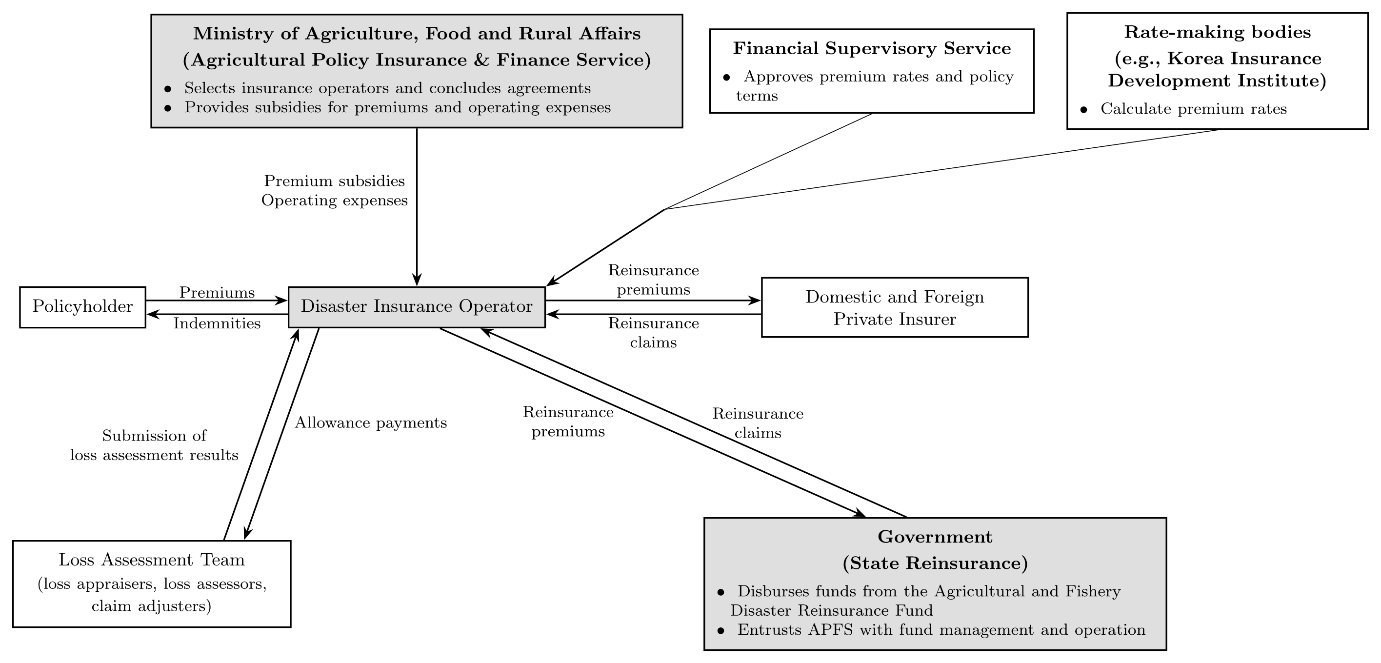
\includegraphics[width=\textwidth]{figures/fig1_organization_fallback.png}%
}
\caption{Organizational Structure of Crop Disaster Insurance in South Korea}\label{fig:organization}
\notes{Arrows indicate payments and the submission of loss assessment results; dashed lines indicate the verification and approval of premium rates and policy terms. Local agricultural cooperatives, which sell contracts on behalf of the operator, are not shown. Adapted from \citet{mafra2025,mafra2026}.}
\end{figure}

NH shares its risk with private reinsurers and with the Agricultural and Fishery Disaster Reinsurance Fund. In 2024, the first-stage shares of the main program's profit-and-loss-sharing arrangement were 10 percent for NH, 40 percent for private reinsurers, and 50 percent for the state \citep[p.~274]{mafra2025}. Additional non-proportional provisions change these shares at higher loss levels, so the first-stage shares do not describe every layer of loss.

The gross premium has two components. The pure premium covers the insured risk and loss-investigation expenses, whereas the premium loading covers specified operating expenses, including delegated selling costs. Under the 2026 rules, the government pays part of the pure premium and all of the loading \citep{mafra2026}. The subsidy rate in equation~\eqref{eq:demand} therefore refers to the pure premium, and the public share of the gross premium is higher than that rate suggests.

\section{Expansion, Enrollment, and Financing}\label{sec:expansion}

The program began with apples and pears in 2001 and covered 78 crops and 94 products in 2026 \citep{mafra2026}. Pilot introduction, expansion of sales regions, and main-program status can fall in different years. The national comparison uses the last pre-pilot year as its reference and ten crop-specific target years beginning with the coded expansion year (Table~\ref{tab:timing}). These milestones distinguish program availability from actual enrollment.

Enrollment, defined as insured area divided by eligible area, rose from 12.5 percent in 2009 to 54.2 percent in 2024 (Figure~\ref{fig:enrollment}). Because eligible area grows whenever crops or regions are added, the national rate reflects program scope as well as take-up. The loss ratio compares claims with premiums for the insurance portfolio; it measures neither income losses of individual farms nor NH's company-wide profitability after reinsurance.

Figure~\ref{fig:premiumshares} shows how the pure premium is financed. In 2024, local governments paid 39.7 percent and policyholders 12.6 percent, leaving 47.7 percent to the central government. Central and local pure-premium support totaled KRW 996.9 billion across 676,226 insured hectares, or approximately KRW 1.47 million per insured hectare \citep{apfs}. This expenditure measure excludes the publicly financed loading; individual transfers vary with insured value, rated risk, and coverage.

\begin{figure}[htbp]
\centering
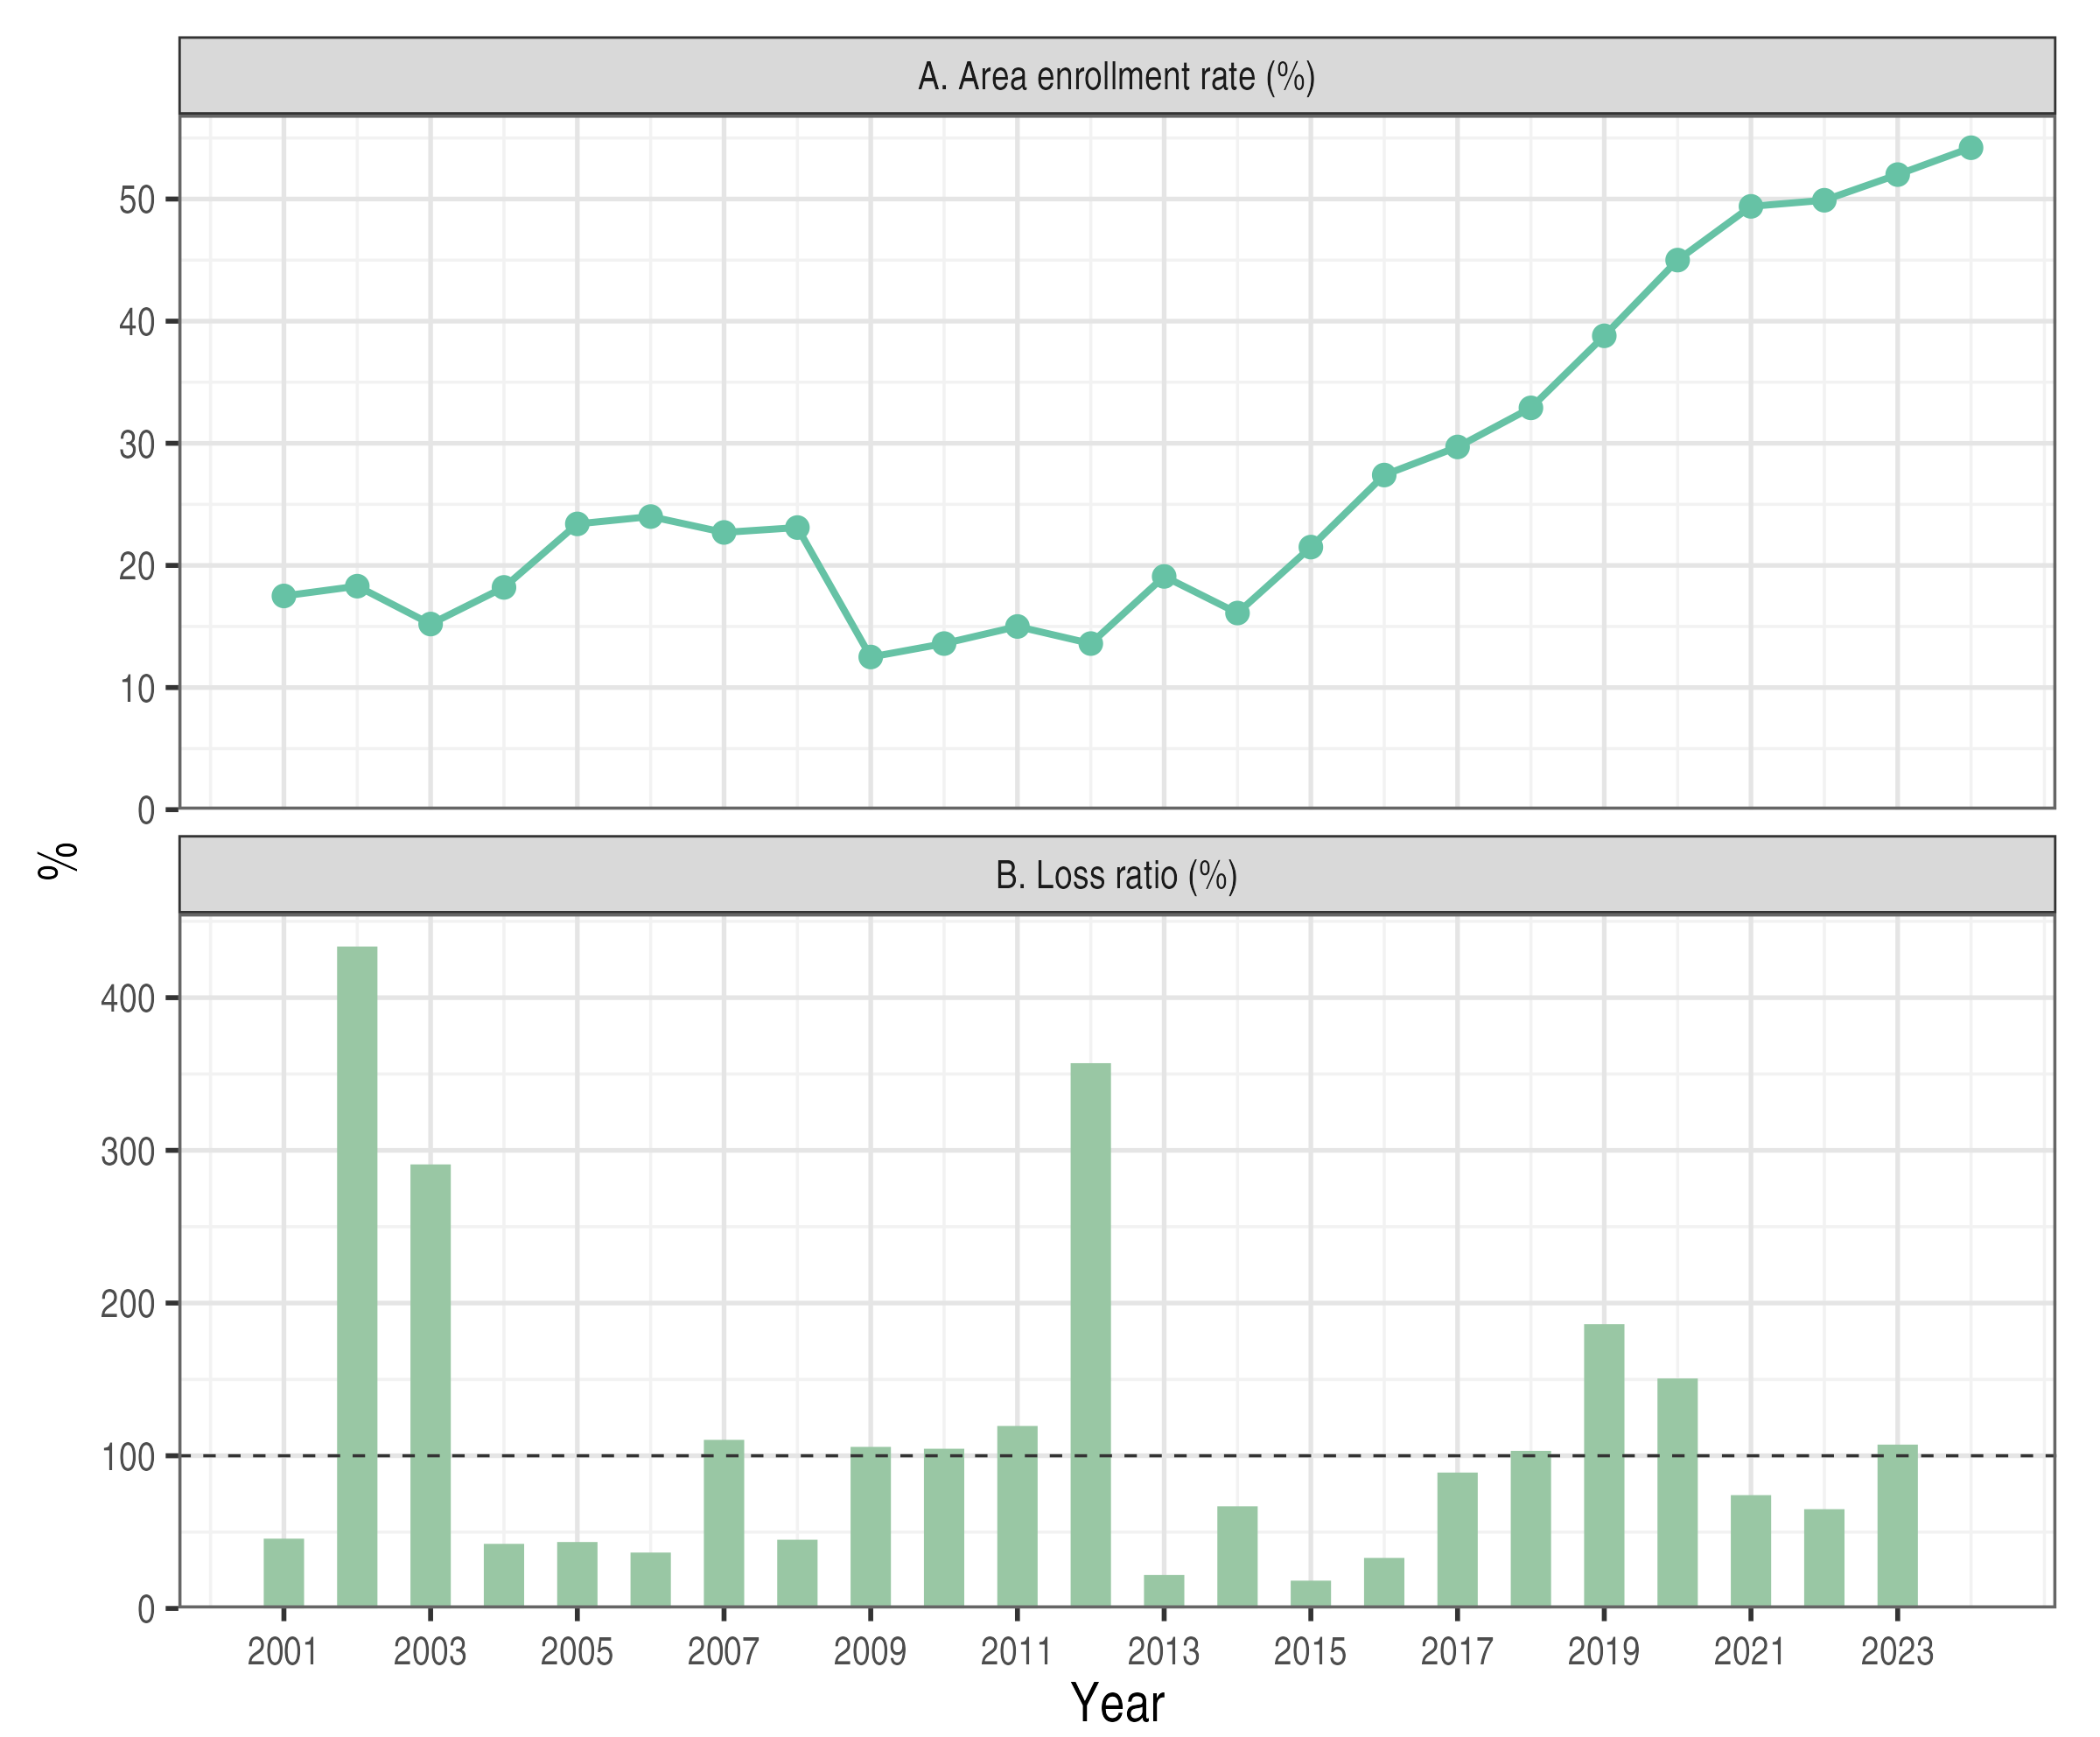
\includegraphics[width=5.0in]{figures/fig2_enrollment_loss_ratio.png}
\caption{National Enrollment Rate and Loss Ratio, 2001-2024}\label{fig:enrollment}
\notes{Enrollment is insured area divided by eligible area. The loss ratio is indemnities divided by premium net of refunds through 2011 and by risk premium from 2012; it is shown through 2023. The horizontal line marks 100 percent. Data from \citet{apfs}.}
\end{figure}

Enrollment also differs sharply across crops (Table~\ref{tab:enrollment}). In 2023, 89.0 percent of eligible apple area and 61.0 percent of eligible rice area were insured, compared with 7.1 percent for sweet potato and 5.4 percent for corn. For the seven annual crops analyzed in Chapter~\ref{ch:results}, the availability of insurance therefore translated into very different degrees of actual coverage.

\begin{figure}[htbp]
\centering
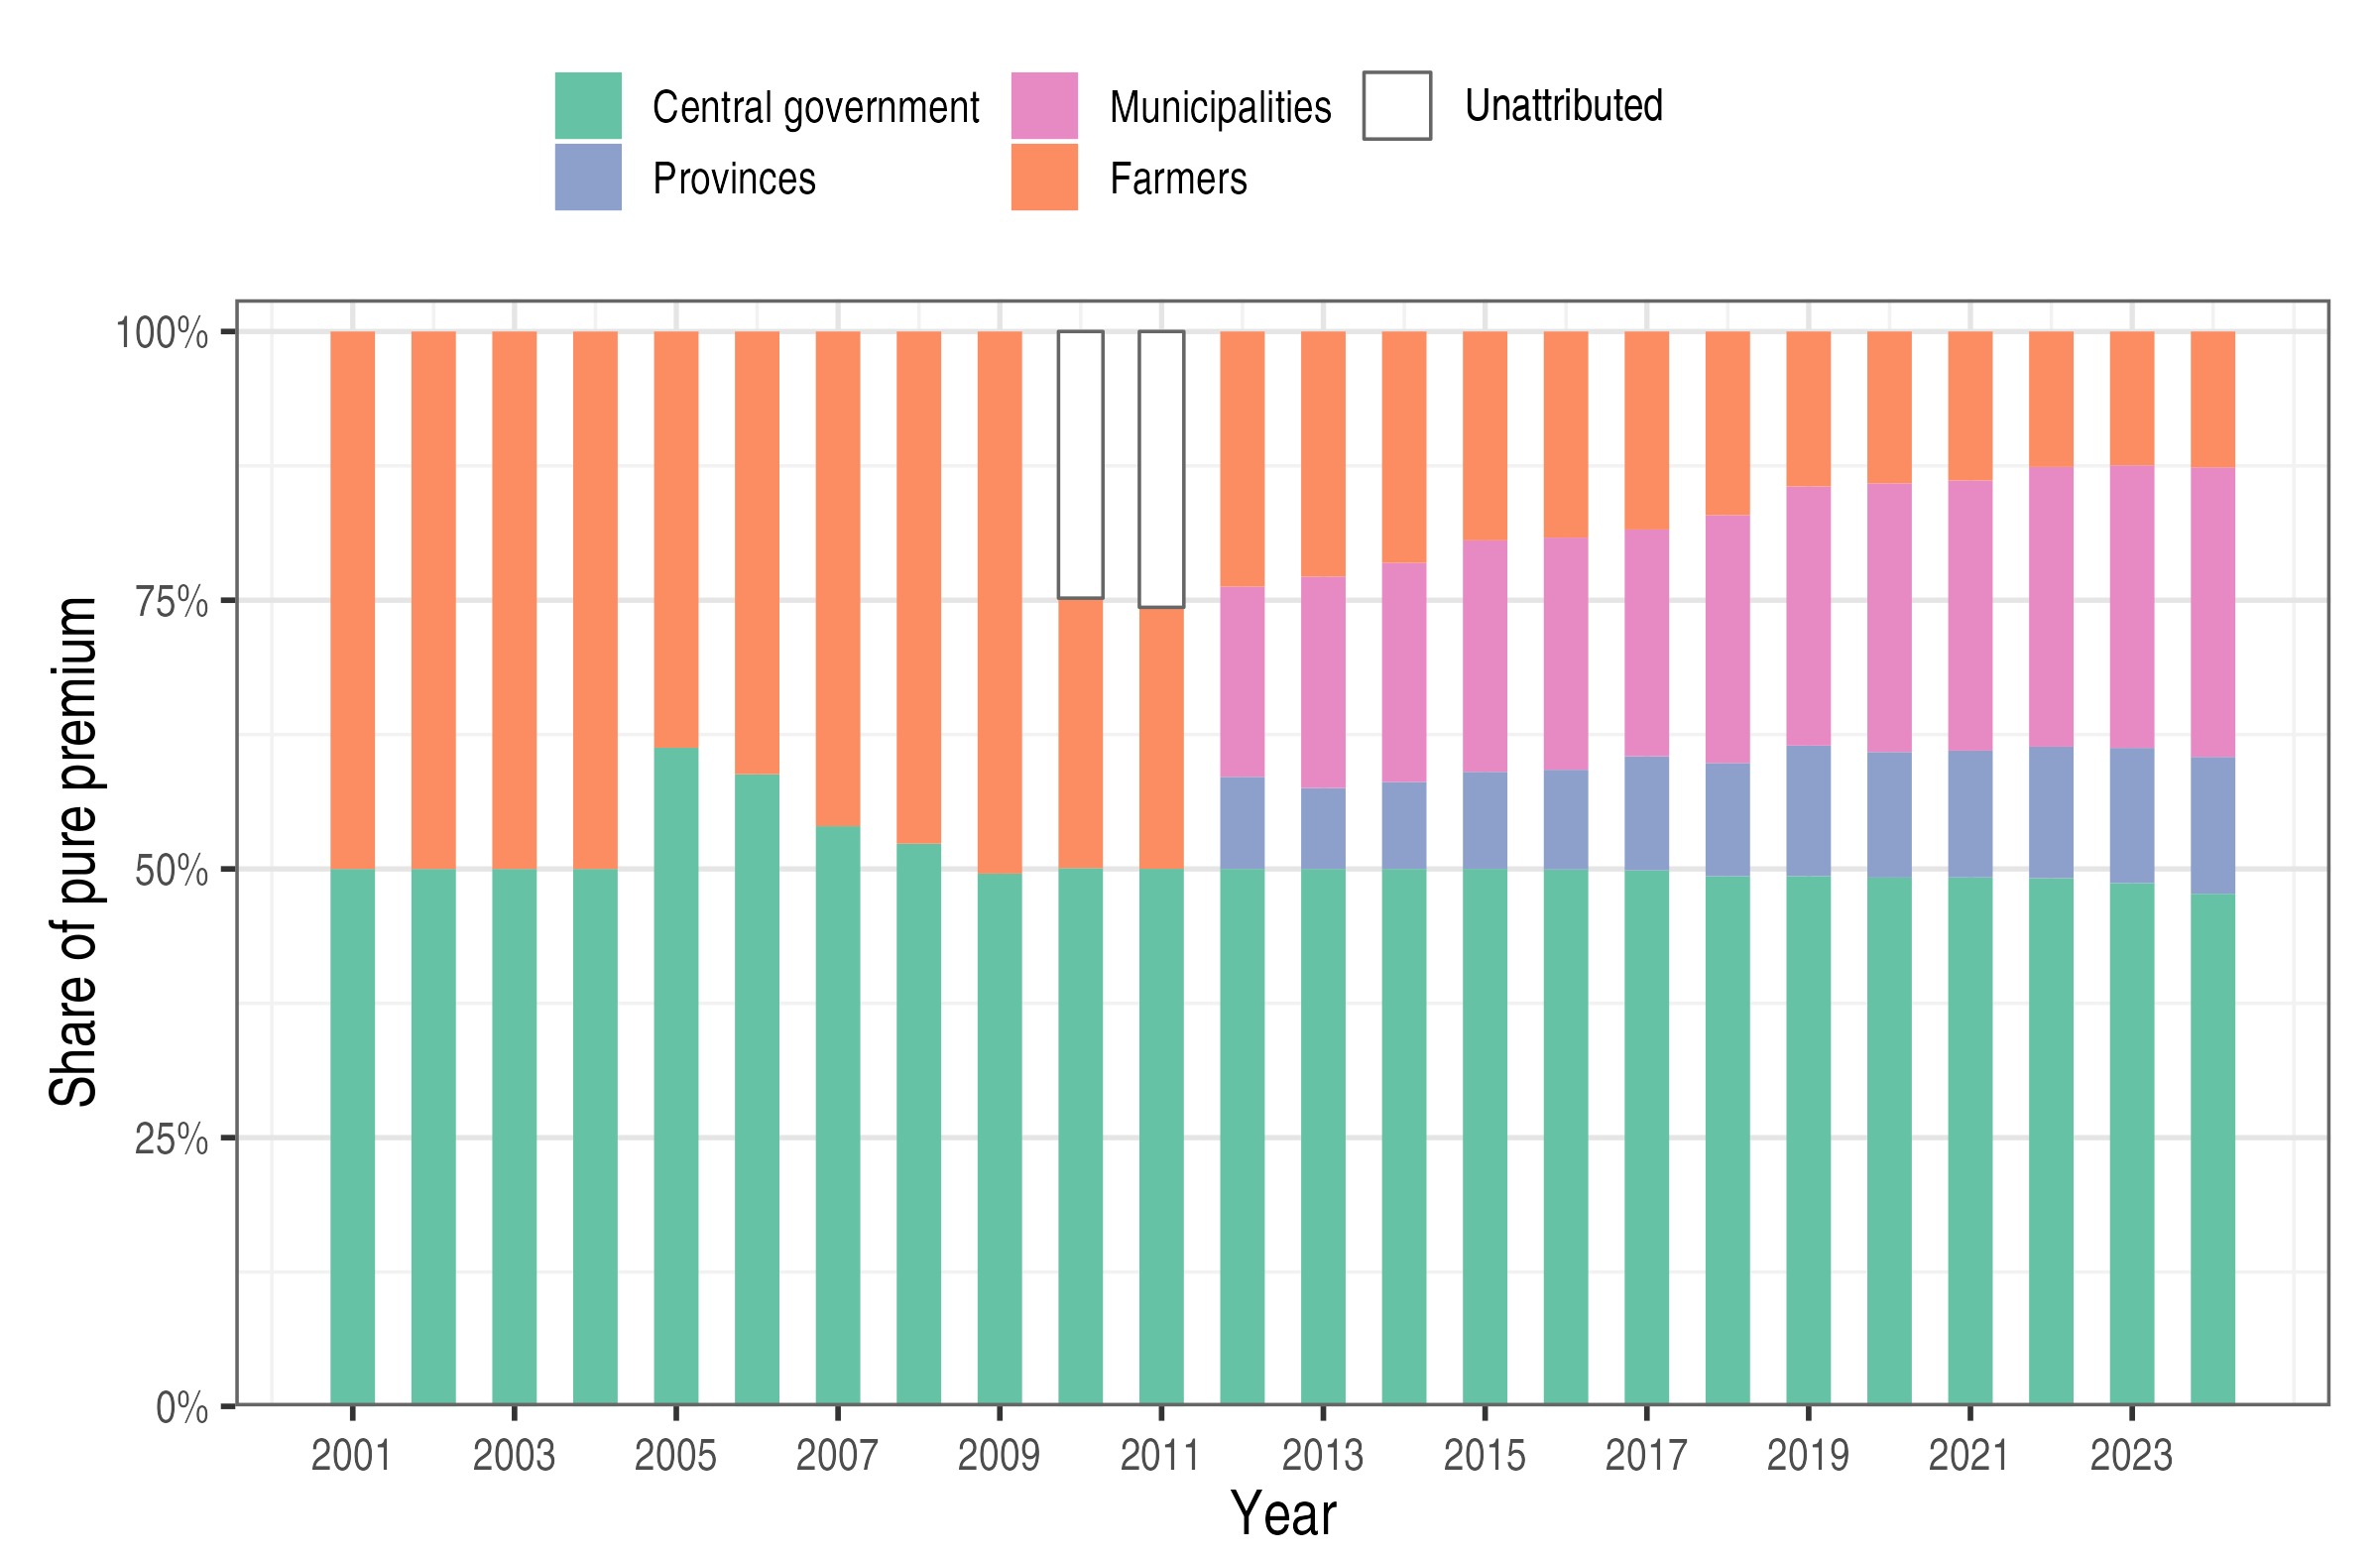
\includegraphics[width=5.4in]{figures/fig3_pure_premium_shares.png}
\caption{Shares of the Pure Premium by Payer, 2001-2024}\label{fig:premiumshares}
\notes{Shares of the reported pure-premium total. Unattributed segments in 2010-2011 are the difference between that total and the identified payer components. The publicly financed loading is excluded. Data from \citet{apfs}.}
\end{figure}

\begin{table}[htbp]
\centering
\caption{Enrollment and Loss Ratios for Selected Crops, 2023}\label{tab:enrollment}
\begin{tabular*}{\textwidth}{@{\extracolsep{\fill}}lcccc}
\toprule
Crop & Eligible area (ha) & Insured area (ha) & Enrollment (\%) & Loss ratio (\%) \\
\midrule
\multicolumn{5}{@{}l}{\textit{Panel A. Rice and major fruits}} \\
Rice          & 725,882 & 443,136 & 61.0 & 103.5 \\
Apple         & 24,945  & 22,209  & 89.0 & 116.1 \\
Pear          & 10,078  & 7,683   & 76.2 & 60.5  \\[4pt]
\multicolumn{5}{@{}l}{\textit{Panel B. Seven annual crops}} \\
Soybean       & 55,326  & 28,649  & 51.8 & 158.9 \\
Onion         & 17,128  & 6,811   & 39.8 & 73.1  \\
Garlic        & 21,110  & 5,936   & 28.1 & 119.0 \\
Red pepper    & 26,126  & 8,522   & 32.6 & 141.7 \\
Spring potato & 3,793   & 727     & 19.2 & 247.8 \\
Sweet potato  & 18,389  & 1,300   & 7.1  & 195.5 \\
Corn          & 14,073  & 764     & 5.4  & 129.2 \\
\bottomrule
\end{tabular*}
\notes{Eligible area can differ from national cultivated area because it depends on each product's sales regions. The loss ratio is indemnities divided by risk premium. Data from \citet{apfs}; author's calculations.}
\end{table}

\section{Related Literature}\label{sec:literature}

Asymmetric information and correlated losses motivate distinct forms of public involvement. Nelson and Loehman \citeyearpar{nelson1987} analyze agricultural insurance contracts under information problems, and \citet{just1999} distinguish actuarial incentives from asymmetric information in participation. Lee and Jung \citeyearpar{leejung2014} examine adverse selection and moral hazard in Korea. Miranda and Glauber \citeyearpar{miranda1997} emphasize systemic risk and reinsurance capacity. \citet{jia2025} show that the appropriate public role depends on loss correlation and relative risk-bearing efficiency. Kang and Chung \citeyearpar{kang2017} examine the implications of Korea's risk-group reinsurance arrangement for the state fund.

Insurance demand reflects differences in risk exposure, financial resources, and the value farmers place on protection, so a common subsidy rate need not generate uniform participation \citep{hazell2017}. Expected disaster relief may also reduce insurance demand through charity hazard \citep{coate1995,raschky2007}. \citet{lusk2017} distinguishes distributional transfers from economic costs. These perspectives separate access, redistribution, and welfare as questions for policy evaluation.

Studies of production responses address different margins. \citet{goodwin2004} and \citet{yu2018} examine acreage responses to U.S. crop insurance and premium subsidies. \citet{han2014} studies production and price effects in Korea, Nam and Ahn \citeyearpar{nam2022} examine input use and farm income, and Lee and Kim \citeyearpar{leekim2026} study insured fruit farms. The present analysis combines an assessment of support instruments with comparisons of aggregate area, yield, and production. Availability-based contrasts differ from estimates of responses among enrolled farms.

Methodologically, timing-specific comparisons avoid using already-exposed units as controls \citep{callaway2021}, but their validity still depends on whether the comparison units trace the untreated path of the treated units. \citet{roth2022} shows that passing a pretrend test does not establish parallel trends and that conditioning on such tests can distort inference. With few treated clusters, cluster-robust and bootstrap inference can be unreliable \citep{cameron2008,mackinnonwebb2018,mackinnon2023,webb2023}, a concern that applies directly to seven treated crops.

\chapter{Assessment of Government Intervention}\label{ch:assessment}

\section{Economic Rationale}\label{sec:rationale}

Each instrument is assessed by the constraint it addresses, the incentives it creates, and the distribution of its costs and benefits. Correlated losses justify public risk-sharing, and the costs of information and delivery justify attention to insurance infrastructure \citep{miranda1997,mahul2010}. Affordability and redistribution can justify premium assistance, but they do not determine a particular rate \citep{hazell2017}. Production can respond to changes in price, access, or risk-bearing under any of the three instruments, so the rollout comparisons in Chapter~\ref{ch:results} test a possible consequence of insurance availability as a package, not the effect of any single instrument.

\section{Premium Subsidies}\label{sec:premium}

Let $P$ be the pure premium per unit of coverage and $s$ the combined national and local subsidy rate, so that the policyholder price is $(1 - s)P$. With coverage demand $D(\cdot)$, coverage purchased without and with support is
\begin{equation}\label{eq:demand}
q_{0} = D(P),\qquad q_{1} = D\bigl((1 - s)P\bigr).
\end{equation}

Figure~\ref{fig:premiumsupport} assumes perfectly elastic supply at $P$. The subsidy raises coverage from $q_{0}$ to $q_{1}$ at a public cost of $sPq_{1}$, of which $sPq_{0}$ is a transfer to purchases that would have occurred without support.

\begin{figure}[htbp]
\centering
\IfFileExists{"insurance graph.tex"}{%
  \adjustbox{max width=\textwidth}{\input{"insurance graph"}}%
}{%
  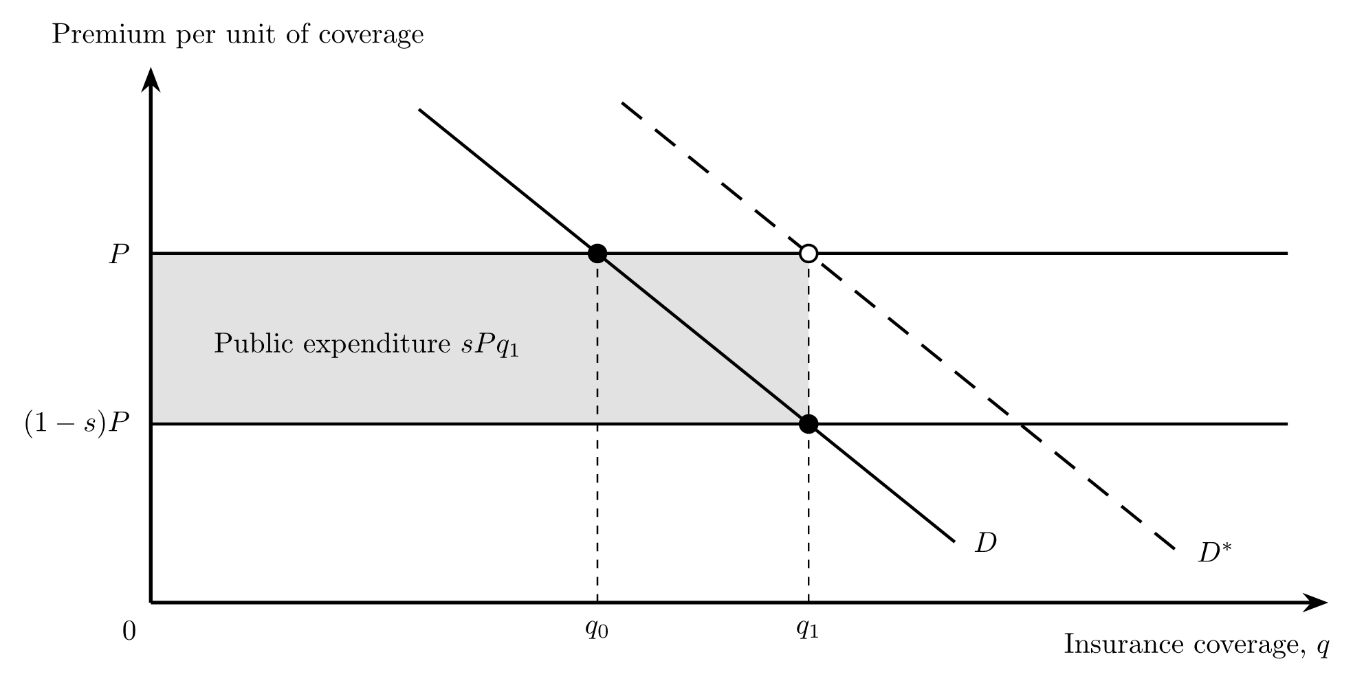
\includegraphics[width=\textwidth]{figures/fig4_premium_support_fallback.png}%
}
\caption{Premium Support and the Demand for Insurance Coverage}\label{fig:premiumsupport}
\notes{$P$ is the pure premium per unit of coverage and $s$ the combined subsidy rate. Supply is perfectly elastic at $P$, and the loading is financed separately. $D$ is observed demand; $D^{*}$ is demand when the value of protection is fully perceived. The shaded rectangle is public pure-premium support, $sPq_{1}$, a transfer rather than a welfare loss. Arbitrary units.}
\end{figure}

Figure~\ref{fig:premiumsupport} is a partial-equilibrium illustration for a given risk class with a fixed premium and loading financed separately. Its shaded rectangle measures a public transfer. If willingness to pay captures protection benefits and $P$ equals marginal resource cost, coverage beyond $q_{0}$ creates an allocative loss. If demand understates those benefits, $D^{*}$ illustrates a possible rationale for additional coverage. Differences in risk preferences, liquidity, and information need not produce the same demand shift, and changes in the insured risk pool can alter premiums. The diagram therefore explains possible mechanisms rather than identifying an optimal subsidy rate or measuring Korean welfare gains.

The 2026 national schedule supports 33-65 percent of the pure premium for specified product-coverage combinations and 50 percent for others, subject to a national subsidy ceiling of KRW 50 million per policyholder per product \citep[p.~2]{mafra2026}. At a fixed subsidy rate, support rises with the eligible premium until this ceiling binds; beyond it, additional premiums receive no additional national subsidy. This limits large transfers but does not target household income. Local assistance must be considered separately. For products sold from July 2026, policyholders with a five-year cumulative loss ratio of at least 500 percent cannot select coverage of 80 percent or higher. Individual loss experience enters premium adjustments for products sold from November 2026 \citep{mafra2026}. Greater risk differentiation can strengthen pricing incentives while reducing affordable protection for repeatedly affected farms.

\section{Administrative Cost Subsidies}\label{sec:administrative}

The 2026 rules distinguish the risk premium and loss-investigation expenses, which together form the pure premium, from the loading, which includes delegated selling and other specified operating costs. Public support covers the loading in full \citep{mafra2026}. Loss-investigation costs should therefore be identified separately when comparing administrative expenditure, rather than counted again as part of the loading. The relevant economic question is whether financing delivers coverage and timely, accurate settlement at a reasonable resource cost.

Comparable indicators require consistent numerators and denominators. Selling and policy-servicing expenditure can be expressed per active contract, and claim-assessment expenditure per completed claim. Product and regional comparisons should also report the operating-cost-to-premium ratio, using a stated premium definition, alongside settlement duration and assessment corrections. Differences in risk prices, claim frequency, product complexity, and geographical dispersion can move these ratios without changing efficiency. Comparisons within similar product and risk categories are consequently more informative than an aggregate international ranking.

Mahul and Stutley \citeyearpar[pp.~84-87]{mahul2010} emphasize the role of low-cost delivery channels. A performance-linked component of administrative payments could reward timely settlement and verified assessment quality, while a separate component maintains access in costly areas. Rewarding closure speed alone could encourage premature or inaccurate settlement. These incentive trade-offs matter independently of whether the aggregate subsidy rises or falls.

\section{State Reinsurance}\label{sec:reinsurance}

State reinsurance provides capacity for correlated losses in exchange for a contingent public liability. A stop-loss contract with attachment point $a$ splits total covered claims $L$ into retained and ceded portions:
\begin{equation}\label{eq:stoploss}
L^{ret} = \min(L,a),\qquad L^{ced} = \max(L - a,0).
\end{equation}

Under a proportional contract, by contrast, the state receives a share of the premium and bears the same share of claims. Korea moved from a stop-loss contract with a 180 percent attachment point in 2005-2013 to a mixed stop-loss and profit-and-loss-sharing arrangement, introduced in 2014 and applied to the whole program from 2019 \citep[pp.~268, 273-274]{mafra2025}. Figure~\ref{fig:reinsurance} contrasts the two benchmark forms. The 50 percent first-stage state share used in Panel B does not fully represent the Korean contract.

In the uncapped stop-loss benchmark, private claims do not rise beyond the attachment point; actual incentives also depend on treaty limits, pricing, and renewal. Proportional sharing preserves marginal private exposure but transfers a share of ordinary losses to the state. The appropriate allocation depends on loss correlation and relative risk-bearing capacity \citep{jia2025}. With reinsurance premium $R$, expressed in the same units as $L$ and $a$, the expected public cost under stop-loss is expected ceded claims minus the premium received:
\begin{equation}\label{eq:publiccost}
E[C] = E\bigl[\max(L - a,0)\bigr] - R.
\end{equation}

Reported crop reinsurance payments over 2005-2024 total KRW 923.8 billion, against receipts of KRW 470.0 billion \citep[p.~269]{mafra2025}. The KRW 453.8 billion difference is a nominal cumulative cash-flow measure, not an inflation-adjusted cost series or the fund's complete financial balance. Actuarial adequacy instead compares premiums with expected losses and risk-bearing costs under each treaty. Comparisons over time must distinguish changes in prices, insured exposure, coverage, contract terms, and settlement dates. Dividing payments by insured hectares alone would not adjust for differences in insured value or loss severity.

\begin{figure}[htbp]
\centering
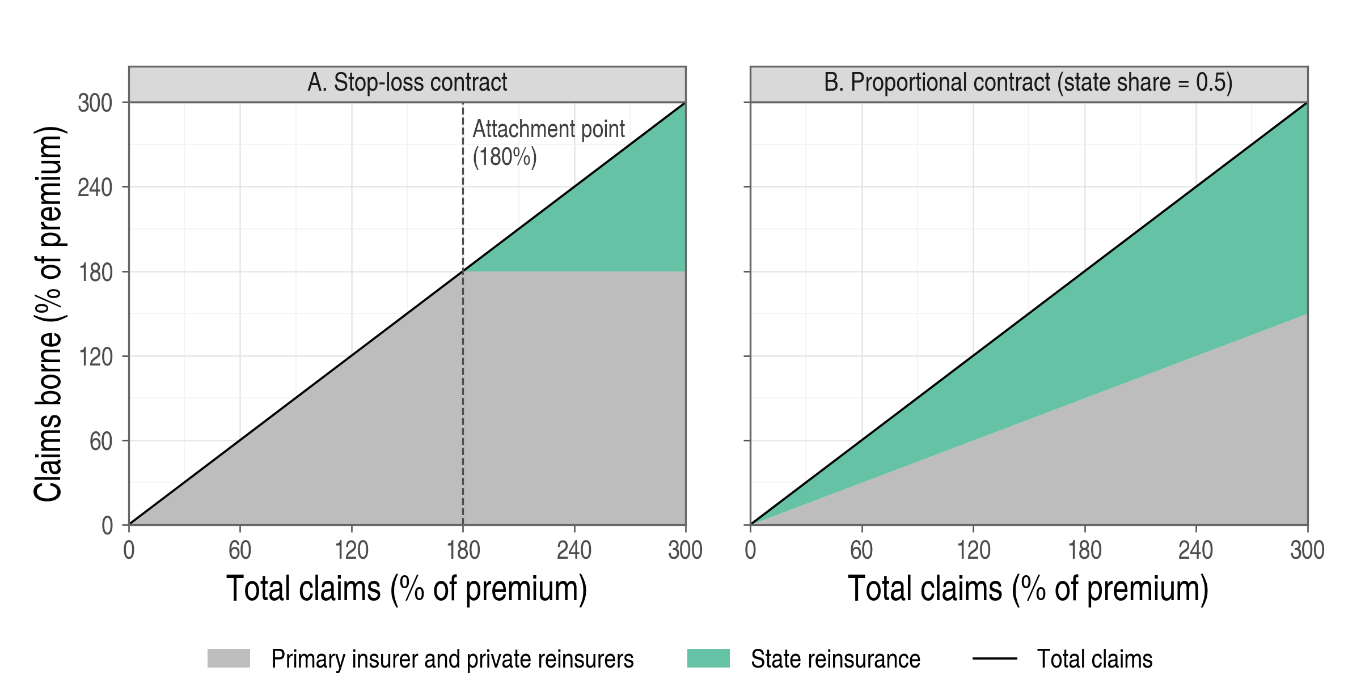
\includegraphics[width=\textwidth]{figures/fig5_reinsurance_allocation.png}
\caption{Allocation of Claims under Stop-Loss and Proportional Reinsurance}\label{fig:reinsurance}
\notes{Both axes express claims as percentages of premium. Panel A uses the 180 percent attachment point reported for 2005-2013 \citep[p.~273]{mafra2025}. Private claims combine those of the operator and private reinsurers. In both panels, the private and state shares are stacked and sum to total claims. Panel B is an illustrative proportional contract without additional layers, premium transfers, expenses, or commissions.}
\end{figure}

A forward-looking assessment should distinguish expected net cost, liquidity when claims fall due, and exposure to severe or consecutive loss years. Each requires the treaty schedule, premiums, reserves, and committed financing. Catastrophe exposure depends on loss dependence as well as frequency and severity \citep{mahul2010,kang2017}. Historical payments should be evaluated under the contracts in force at the time rather than retrospectively applying current sharing rates.

\chapter{Data and Empirical Strategy}\label{ch:data}

\section{Data and Summary Statistics}\label{sec:data}

The national data are a crop-year panel of 43 crop or crop-form series from the Crop Production Survey \citep{statkorea_nd}, analyzed over 1991-2024. Cultivated area is in hectares, yield in kilograms per 10 ares, and production in metric tonnes. One hectare contains ten units of 10 ares, and one tonne contains 1,000 kilograms. Thus production equals area \texttimes{} yield \texttimes{} 10/1,000, or area \texttimes{} yield / 100, up to reporting and rounding differences. Equivalently, 100 kg/10a equals 1 tonne/ha. With identical observations and weights, the log production contrast is approximately the sum of the log area and yield contrasts. This is an accounting decomposition; average yield can reflect both productivity and the composition of cultivated land.

Exposure is defined by the availability of insurance, not by enrollment, and national totals include insured and uninsured farms. Two changes in survey methods affect comparability: sweet potato moved to administrative reporting in 2005, and spring napa cabbage and spring radish moved to a sample survey in 2012 \citep{statkorea2014}.

Table~\ref{tab:summary} reports the mean, standard deviation, and range of the unique crop-year observations entering the main comparison. Treated crops are on average about three times larger in cultivated area. These statistics describe levels and dispersion. Differences in observed pre-pilot changes are examined in Section~\ref{sec:comparability}; similar means or a log transformation would not establish parallel untreated trends.

\begin{table}[htbp]
\centering
\caption{Summary Statistics}\label{tab:summary}
\begin{tabular*}{\textwidth}{@{\extracolsep{\fill}}lrrrrcc}
\toprule
 & Mean & S.D. & Min. & Max. & Obs. & Crops \\
\midrule
\multicolumn{7}{@{}l}{\textit{Panel A. Area (ha)}} \\
Treated, reference year     & 31,958 & 24,132 & 13,033 & 76,267 & 7   & 7  \\
Treated, target years       & 26,991 & 15,482 & 13,017 & 80,842 & 70  & 7  \\
Comparison, reference years & 9,775  & 9,659  & 1,062  & 34,875 & 66  & 22 \\
Comparison, target years    & 9,083  & 10,014 & 619    & 45,474 & 218 & 22 \\[4pt]
\multicolumn{7}{@{}l}{\textit{Panel B. Yield (kg/10a)}} \\
Treated, reference year     & 1,934 & 2,311 & 150 & 6,725  & 7   & 7  \\
Treated, target years       & 1,856 & 2,161 & 147 & 8,541  & 70  & 7  \\
Comparison, reference years & 2,488 & 2,696 & 37  & 10,946 & 66  & 22 \\
Comparison, target years    & 2,335 & 2,757 & 30  & 11,286 & 218 & 22 \\[4pt]
\multicolumn{7}{@{}l}{\textit{Panel C. Production (t)}} \\
Treated, reference year     & 350,922 & 323,462 & 92,830 & 1,035,076 & 7   & 7  \\
Treated, target years       & 381,113 & 424,756 & 55,714 & 1,594,450 & 70  & 7  \\
Comparison, reference years & 208,852 & 330,283 & 1,589  & 1,582,966 & 66  & 22 \\
Comparison, target years    & 163,544 & 295,436 & 1,598  & 1,698,463 & 218 & 22 \\
\bottomrule
\end{tabular*}
\notes{Statistics are computed over unique crop-year observations that enter the main comparison. S.D. is the standard deviation of observations. Reference years are crop-specific; target years are the ten years beginning with the coded expansion year.}
\end{table}

\section{Sample and Exposure Timing}\label{sec:sample}

The treated sample consists of seven annual crops (soybean, onion, sweet potato, corn, garlic, spring potato, and red pepper), each with a continuous series from 1991, a dated pilot, and ten observed years after expansion. Fruit crops are excluded because orchard area and perennial production respond on different time scales, and autumn potato is excluded because its milestones are not reported separately from other potato forms. Rice is analyzed separately through its municipal rollout (Section~\ref{sec:rice_design}).

Table~\ref{tab:timing} reports the timing used to organize the comparisons. The pilot year marks regional availability, and the coded expansion year begins the ten target years. Neither implies universal enrollment or geographical coverage. Historical announcement dates are converted into harvest years using recent sales calendars, creating timing uncertainty. Spring potato remained restricted to selected regions in 2023-2024 \citep{mafra2024,mafra2025}, so its coded expansion year should not be interpreted as nationwide availability. Alternative milestone definitions are examined in Table~\ref{tab:sensitivity}.

\begin{table}[htbp]
\centering
\caption{Insurance Timing for the Seven Annual Crops}\label{tab:timing}
\begin{tabular*}{\textwidth}{@{\extracolsep{\fill}}lccccc}
\toprule
Crop & \shortstack{Pilot\\year} & \shortstack{Expansion\\year} & \shortstack{Product-table\\year} & \shortstack{Reference\\year} & \shortstack{Transition\\years} \\
\midrule
Soybean       & 2008 & 2012 & 2011 & 2007 & 4 \\
Onion         & 2009 & 2012 & 2011 & 2008 & 3 \\
Sweet potato  & 2009 & 2013 & 2012 & 2008 & 4 \\
Corn          & 2009 & 2013 & 2012 & 2008 & 4 \\
Garlic        & 2010 & 2013 & 2012 & 2009 & 3 \\
Spring potato & 2008 & 2013 & 2011 & 2007 & 5 \\
Red pepper    & 2008 & 2015 & 2014 & 2007 & 7 \\
\bottomrule
\end{tabular*}
\notes{Pilot and expansion years follow the milestone sequence described in Section~\ref{sec:expansion}. Reference year is the pilot year minus one. Transition years run from the pilot year to the year before expansion. Product-table years are an alternative milestone used in Table~\ref{tab:sensitivity}. Data from \citet[pp.~37, 44, 46]{mafra2025}.}
\end{table}

The candidate comparison pool contains 24 annual crop series, of which 22 contribute to the main contrast. A crop is eligible as a comparison only if both its reference and target observations precede its own pilot, or if it has no pilot by 2024. Because all seven treated crops entered pilots by 2010, before the earliest target year of 2012, they never serve as comparisons for one another in the main post-period contrasts.

\section{National Crop Comparisons}\label{sec:national_design}

The national analysis constructs crop-specific difference-in-differences contrasts and averages them across seven crops and ten target years. Let $p_{i}$ be the pilot year, $g_{i}$ the expansion year, and $b_{i} = p_{i} - 1$ the reference year of treated crop $i$. At event year $e$, the target year is $g_{i} + e$, and the comparison set $C_{i,e}$ contains the $n_{i,e}$ crops observed and not yet exposed in both $b_{i}$ and $g_{i} + e$. For a log outcome $y$, the crop-event contrast is
\begin{equation}\label{eq:contrast}
\widehat{\delta}_{i,e} = \left( y_{i,g_{i} + e} - y_{i,b_{i}} \right) - \frac{1}{n_{i,e}}\sum_{j \in C_{i,e}}\left( y_{j,g_{i} + e} - y_{j,b_{i}} \right)
\end{equation}
and the contrasts are averaged with equal weights across crops and event years:
\begin{equation}\label{eq:average}
\widehat{\theta}_{e} = \frac{1}{7}\sum_{i = 1}^{7}\widehat{\delta}_{i,e},\qquad \widehat{\theta} = \frac{1}{10}\sum_{e = 0}^{9}\widehat{\theta}_{e}.
\end{equation}

The first term in equation~\eqref{eq:contrast} is the log growth of the treated crop from its reference year, and the second is the average log growth of its comparison crops over the same interval. Each contrast is therefore a difference in log changes from the reference year: the growth of the treated crop in excess of the growth of crops not yet insured. The statistic $\widehat{\theta}$ averages these net growth rates over seven crops and ten target years, and multiplied by 100 it approximates a difference in percentage growth. Because the reference year precedes the pilot, $\widehat{\theta}$ covers the pilot transition as well as the period after expansion.

As an alternative aggregation, crops are weighted by their mean cultivated area in 2003-2007, before the earliest pilot:
\begin{equation}\label{eq:areaweights}
\widehat{\theta}^{A} = \frac{1}{10}\sum_{e = 0}^{9}\sum_{i = 1}^{7}w_{i}^{A}\,\widehat{\delta}_{i,e},\qquad w_{i}^{A} = \frac{\bar{A}_{i}^{pre}}{\sum_{k = 1}^{7}\bar{A}_{k}^{pre}}
\end{equation}

Event-time contrasts use the pilot year to locate observations on the horizontal axis while retaining the last pre-pilot year as the reference observation. For each event year, equation~\eqref{eq:contrast} compares the treated crop's change with that of eligible comparison crops, and the seven contrasts are averaged equally. The last pre-pilot contrast is zero by construction. Earlier contrasts describe observed pre-pilot differences; their joint test assesses whether nine contrasts are zero. Neither a small contrast nor a non-rejection establishes parallel untreated trends. Post-pilot contrasts include the transition before coded expansion.

\section{Municipal Rice Comparison}\label{sec:rice_design}

Rice insurance was first offered in 20 municipalities in 2009, with ten further municipalities added in 2011 \citep{choi2010,mifaff2011}. Both cohorts were designated as major producing areas. Later entrants provide a comparison for early entrants through 2010, before their own eligibility. A shared designation holds some features of program selection constant but does not make rollout timing random. Section~\ref{sec:rice_results} compares observed pre-pilot characteristics and paths.

The outcome is log paddy-rice planted area for 2000-2010 from the Crop Production Survey. Restricting the sample to mainland municipalities with complete, boundary-consistent series leaves 17 early and nine later entrants, or 286 municipality-years. The estimating equation is
\begin{equation}\label{eq:rice}
\ln A_{mt} = \alpha_{m} + \lambda_{t} + \beta D_{mt} + \varepsilon_{mt}
\end{equation}
where $A_{mt}$ is planted area in municipality $m$ and year $t$, $\alpha_{m}$ and $\lambda_{t}$ are municipality and year fixed effects, and $D_{mt}$ equals one for early entrants in 2009-2010. Municipality fixed effects absorb time-invariant differences such as soil quality, irrigation infrastructure, and proximity to markets; year fixed effects absorb national shocks such as rice prices and weather common to all municipalities.

\section{Identification, Inference, and Scope}\label{sec:identification}

A causal interpretation requires that treated and comparison units would have followed parallel changes without insurance, with correctly dated exposure and no anticipation or spillovers. For the national comparison, crop substitution or common-market responses could affect comparison crops even before their own eligibility. Pre-pilot paths and group characteristics assess observed comparability but cannot establish the untreated post-pilot path. The rice comparison holds crop identity fixed; regional weather, investment, and other time-varying local conditions may nevertheless differ between cohorts.

National uncertainty is summarized with crop-level scores and independent Webb six-point multipliers (Appendix~\ref{app:inference}). The procedure is neither null-imposed nor studentized, and its small-sample coverage is not established. Webb weights alone do not resolve few-treated-cluster problems \citep{mackinnonwebb2018}. Municipal inference uses a null-imposed, CR1-studentized wild cluster bootstrap with Webb weights and 9,999 draws, with intervals obtained by test inversion \citep{cameron2008,webb2023}. Finite-sample concerns remain with 26 municipality clusters, including nine comparisons. Tables report standard errors in parentheses, 95 percent intervals in brackets, and * for p < 0.10, ** for p < 0.05, and *** for p < 0.01. Statistical significance otherwise refers to the 5 percent level.

Uncertainty and identification are separate considerations. A wide interval limits precision even under valid identifying assumptions; a narrow interval cannot resolve a biased comparison.\footnote{A normal-approximation benchmark, treating the reported standard errors as fixed (0.159 for the national production contrast and 0.022 for the rice estimate), gives minimum detectable effects of approximately 0.45 and 0.06 log points for 80 percent power at a two-sided 5 percent level. These calculations do not establish the power of the bootstrap procedures used here.} The national intervals are exploratory because the score procedure's nominal coverage is uncertain. Alternative reference periods, comparison pools, and weights were examined after the main results were known and are reported as sensitivity analyses.

\chapter{Results}\label{ch:results}

\section{Pre-Pilot Trajectories}\label{sec:prepilot}

Figure~\ref{fig:eventtime} reports event-time contrasts relative to the last pre-pilot year. Each point subtracts the comparison crops' mean log change from the treated crops' mean log change over the same interval. Pre-pilot contrasts near zero would be consistent with parallel observed changes, whereas systematic differences raise concerns about the national comparison. The reference contrast is fixed at zero by construction.

The pre-pilot yield contrasts lie between approximately \textminus 0.04 and 0.03 log points. The joint test has p = 0.88 and does not reject at the 5 percent level. Its power and calibration are limited by the small number of treated crops.

Area and production show more pronounced pre-pilot differences. Their contrasts are approximately \textminus 0.2 log points in earlier years and closer to zero near the reference year, indicating that treated crops gained relative to their comparisons before insurance. The exploratory joint p-values are 0.06 for area and 0.03 for production: only production crosses the stated 5 percent threshold. Both paths remain relevant to assessing comparability, regardless of that threshold. Their similarity is consistent with the accounting relationship between area, yield, and production.

\begin{figure}[htbp]
\centering
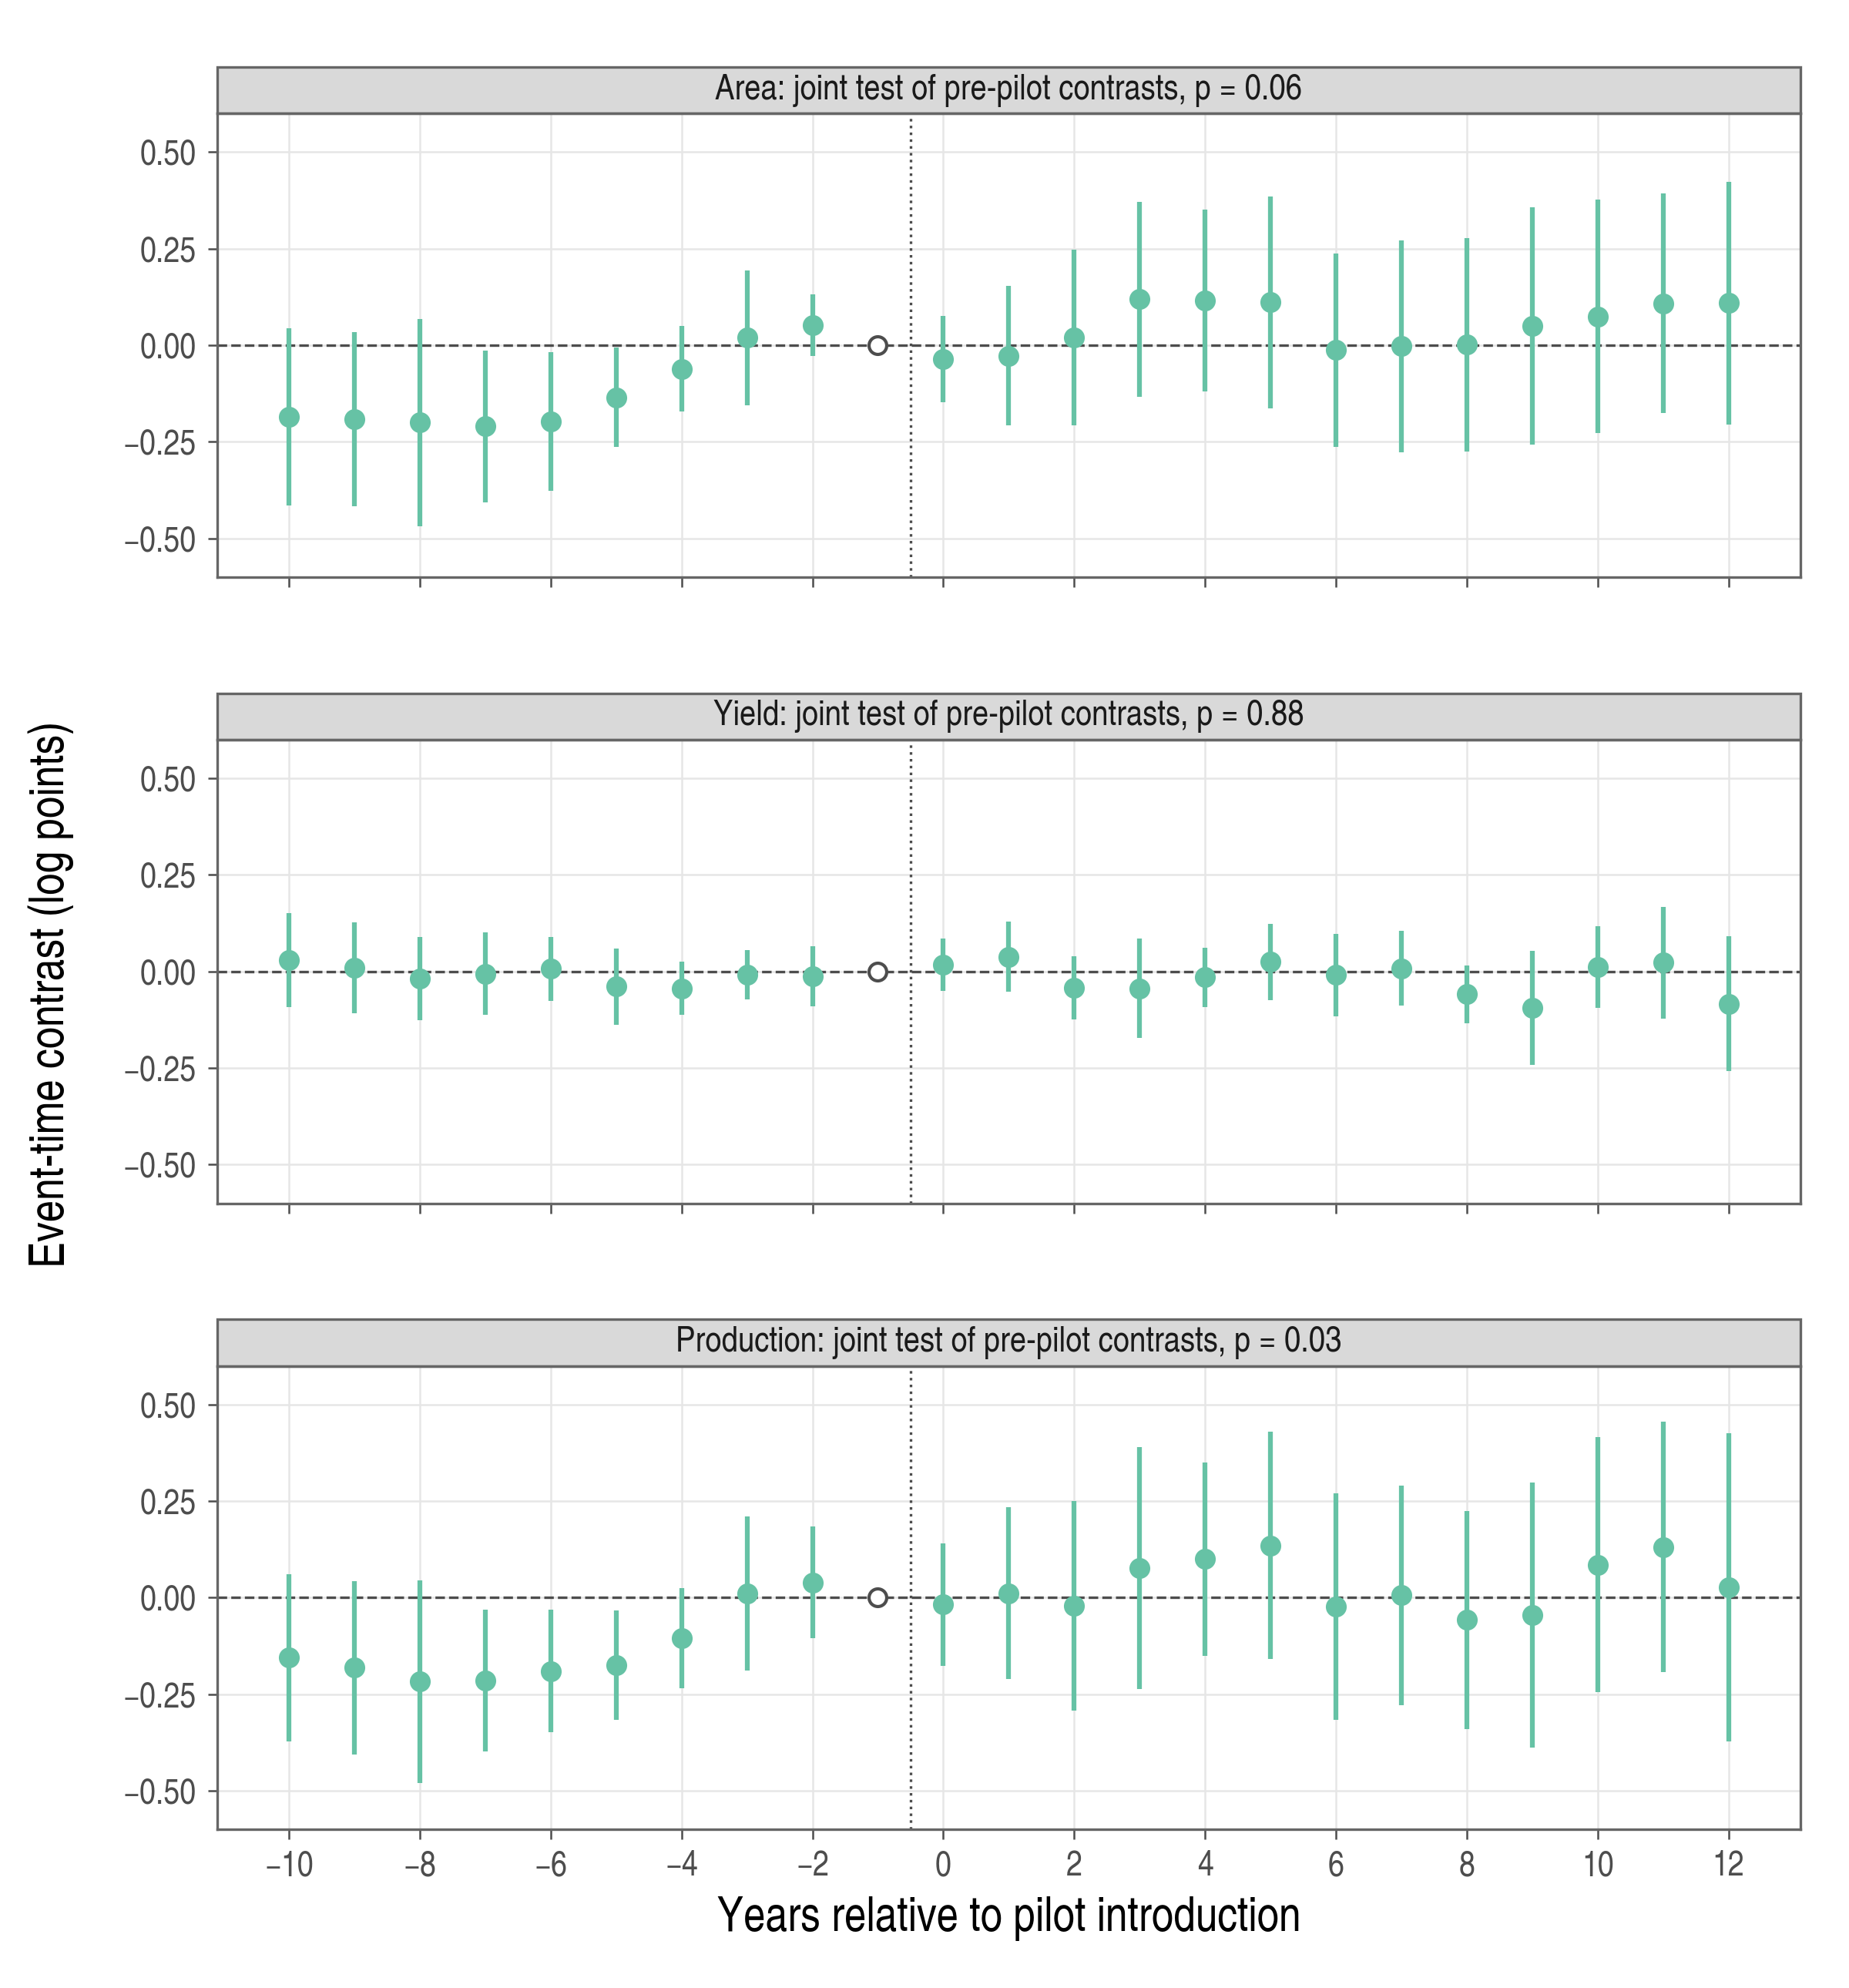
\includegraphics[width=5.40in]{figures/fig6_event_time_contrasts.png}
\caption{Event-Time Contrasts for Cultivated Area, Yield, and Production}\label{fig:eventtime}
\notes{Event-time contrasts relative to the last pre-pilot year (open circle), averaged over the seven treated crops. Bars are 95 percent intervals from 9,999 Webb multiplier draws (Appendix~\ref{app:inference}). The vertical dotted line separates pre-pilot and post-pilot years; post-pilot years include the transition years between the pilot and expansion.}
\end{figure}

Area and production gained relative to comparison crops before the pilots. A reference year close to introduction consequently measures subsequent changes from a later point in that divergence. Section~\ref{sec:sensitivity} examines how alternative reference periods change the reported contrasts.

\section{Aggregate and Crop-Level Contrasts}\label{sec:aggregate}

Table~\ref{tab:main} reports the main contrasts for the full comparison pool and for a pool that excludes spring napa cabbage and spring radish, whose survey method changed in 2012 and whose relation to separately reported winter series from 2014 is undocumented.

\begin{table}[htbp]
\centering
\caption{Mean Post-Period Contrasts}\label{tab:main}
\begin{tabular*}{\textwidth}{@{\extracolsep{\fill}}lccc}
\toprule
 & (1) & (2) & (3) \\
 & Area & Yield & Production \\
\midrule
\multicolumn{4}{@{}l}{\textit{Panel A. Full comparison pool}} \\
Mean contrast      & 0.048            & \textminus 0.028          & 0.020 \\
                   & (0.139)          & (0.055)           & (0.159) \\
                   & [\textminus 0.213, 0.310] & [\textminus 0.133, 0.076] & [\textminus 0.277, 0.317] \\
Comparison series  & 22               & 22                & 22 \\[4pt]
\multicolumn{4}{@{}l}{\textit{Panel B. Excluding two spring series}} \\
Mean contrast      & \textminus 0.041          & \textminus 0.032          & \textminus 0.074 \\
                   & (0.134)          & (0.058)           & (0.157) \\
                   & [\textminus 0.293, 0.210] & [\textminus 0.144, 0.080] & [\textminus 0.369, 0.221] \\
Comparison series  & 20               & 20                & 20 \\
\bottomrule
\end{tabular*}
\notes{Log outcomes; seven treated crops; ten target years. Target years begin with the coded expansion year, whereas Figure~\ref{fig:eventtime} indexes time relative to pilot introduction. Panel B excludes spring napa cabbage and spring radish. Score-based standard errors in parentheses and 95 percent intervals in brackets from 9,999 Webb multiplier draws; their nominal coverage is not established for this design (Appendix~\ref{app:inference}). * p < 0.10, ** p < 0.05, *** p < 0.01.}
\end{table}

With the full comparison pool, the mean contrasts are 0.048 for area, \textminus 0.028 for yield, and 0.020 for production (p = 0.73, 0.61, and 0.90). Excluding the two spring series changes them to \textminus 0.041, \textminus 0.032, and \textminus 0.074. Area and production change sign, while yield changes little. The full-pool production interval, approximately [\textminus 0.28, 0.32] log points, includes substantial decreases and increases.

Figure~\ref{fig:cropcontrasts} decomposes the aggregate into the seven crop-specific means.

\begin{figure}[htbp]
\centering
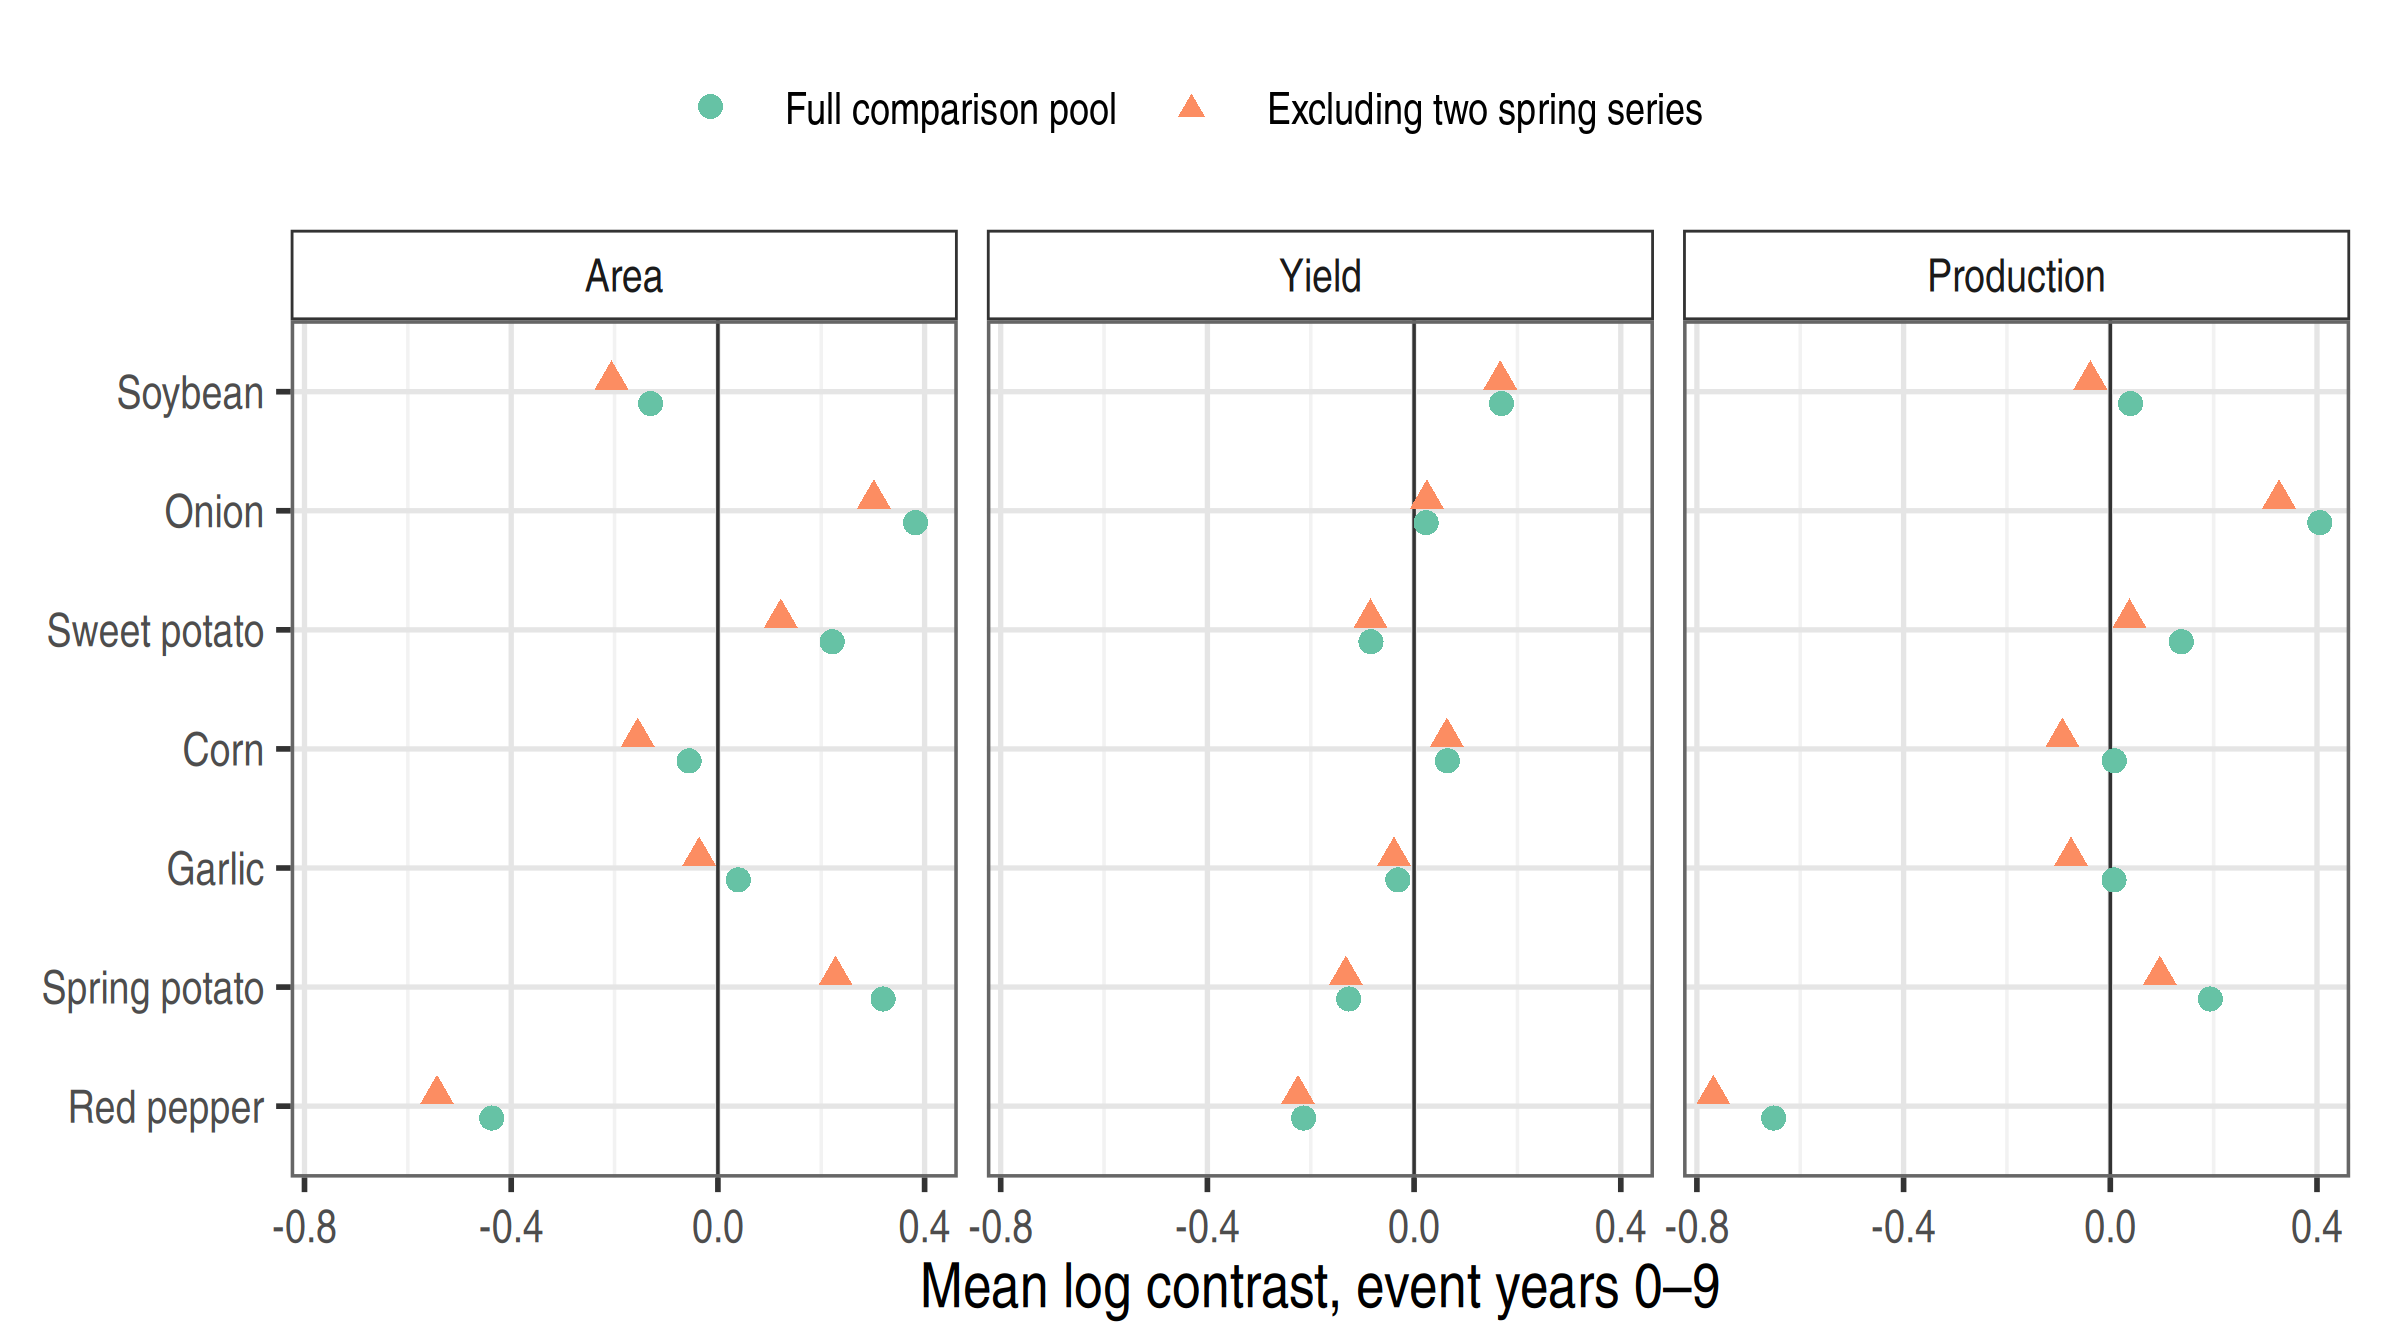
\includegraphics[width=\textwidth]{figures/fig7_crop_contrasts.png}
\caption{Mean Contrasts by Treated Crop}\label{fig:cropcontrasts}
\notes{Each point averages ten crop-specific contrasts. Circles use the full comparison pool, and triangles exclude spring napa cabbage and spring radish. Log points.}
\end{figure}

The small aggregate combines large offsetting contrasts. Production contrasts are 0.406 for onion and 0.193 for spring potato but \textminus 0.651 for red pepper. With equal weights, their respective contributions are approximately 0.058, 0.028, and \textminus 0.093 log points. Omitting one crop at a time moves the aggregate between \textminus 0.044 and 0.132 (Appendix Table~\ref{tab:leaveoneout}). This sensitivity establishes the influence of individual crops, without identifying whether their movements reflect insurance, other shocks, or differences in untreated trends.

\section{Sensitivity to Comparison Choices}\label{sec:sensitivity}

Table~\ref{tab:sensitivity} varies one element of the comparison at a time, keeping the format of Table~\ref{tab:main}.

\begin{table}[htbp]
\centering
\caption{Sensitivity to the Reference Period, Comparison Crops, and Timing}\label{tab:sensitivity}
\begin{tabular*}{\textwidth}{@{\extracolsep{\fill}}lccc}
\toprule
 & (1) & (2) & (3) \\
 & Area & Yield & Production \\
\midrule
\multicolumn{4}{@{}l}{\textit{Panel A. Reference period: mean of last five pre-pilot years}} \\
Contrast & 0.075            & \textminus 0.008          & 0.067 \\
         & (0.150)          & (0.050)           & (0.164) \\
         & [\textminus 0.210, 0.361] & [\textminus 0.105, 0.088] & [\textminus 0.244, 0.378] \\[4pt]
\multicolumn{4}{@{}l}{\textit{Panel B. Reference period: mean of all pre-pilot years}} \\
Contrast & 0.264            & \textminus 0.036          & 0.228 \\
         & (0.184)          & (0.071)           & (0.191) \\
         & [\textminus 0.082, 0.611] & [\textminus 0.170, 0.097] & [\textminus 0.129, 0.585] \\[4pt]
\multicolumn{4}{@{}l}{\textit{Panel C. Comparison crops: field crops only}} \\
Contrast & \textminus 0.054          & \textminus 0.037          & \textminus 0.091 \\
         & (0.187)          & (0.081)           & (0.235) \\
         & [\textminus 0.402, 0.294] & [\textminus 0.190, 0.116] & [\textminus 0.536, 0.354] \\[4pt]
\multicolumn{4}{@{}l}{\textit{Panel D. Comparison crops: excluding uncertain seasonal forms}} \\
Contrast & \textminus 0.082          & \textminus 0.022          & \textminus 0.105 \\
         & (0.154)          & (0.066)           & (0.184) \\
         & [\textminus 0.373, 0.208] & [\textminus 0.146, 0.101] & [\textminus 0.453, 0.243] \\[4pt]
\multicolumn{4}{@{}l}{\textit{Panel E. Timing: product-table years}} \\
Contrast & 0.062            & \textminus 0.025          & 0.036 \\
         & (0.135)          & (0.051)           & (0.153) \\
         & [\textminus 0.192, 0.315] & [\textminus 0.122, 0.072] & [\textminus 0.250, 0.323] \\[4pt]
\multicolumn{4}{@{}l}{\textit{Panel F. Timing: pilot year as start of exposure}} \\
Contrast & 0.034            & \textminus 0.018          & 0.017 \\
         & (0.113)          & (0.045)           & (0.128) \\
         & [\textminus 0.178, 0.247] & [\textminus 0.102, 0.066] & [\textminus 0.224, 0.258] \\
\bottomrule
\end{tabular*}
\notes{Log outcomes; seven treated crops; ten target years; full comparison pool unless stated. Score-based standard errors in parentheses and 95 percent intervals in brackets from 9,999 Webb multiplier draws (Appendix~\ref{app:inference}). * p < 0.10, ** p < 0.05, *** p < 0.01. The main specification is reported in Table~\ref{tab:main}, Panel A. Multi-year references require comparison crops to be observed and not yet exposed in every reference year. Panel D excludes napa cabbage and radish forms, carrot, and green onions, whose survey definitions are uncertain. Panel F dates exposure from the pilot rather than from expansion.}
\end{table}

No specification yields a statistically significant contrast; the smallest p-value, 0.144, belongs to the area contrast with all pre-pilot years as the reference. The reference period and comparison pool nevertheless move the point estimates considerably. Earlier reference periods raise the production contrast to 0.067 and 0.228, as the pre-pilot contrasts in Figure~\ref{fig:eventtime} predict: a longer reference window places the baseline in years when the treated crops were further behind. Restricting the comparison pool lowers the production contrast to \textminus 0.091 or \textminus 0.105, while the timing changes matter less (0.036 and 0.017). The standard errors, between 0.11 and 0.24 for area and production, are large relative to every point estimate, so the specifications differ more in where they center the estimate than in what they can rule out.

Weighting crops by pre-pilot area changes the production contrast from 0.020 to \textminus 0.093, and from \textminus 0.074 to \textminus 0.185 without the two spring series (Table~\ref{tab:areaweights}). Soybean and red pepper receive 61 percent of the weight, whereas onion and spring potato, whose contrasts are positive, receive less. None of the weighted contrasts is statistically significant, and the area-weighted figure is a different summary of the same crop contrasts rather than the percentage change in national production.

\begin{table}[htbp]
\centering
\caption{Contrasts under Pre-Pilot Area Weights}\label{tab:areaweights}
\begin{tabular*}{\textwidth}{@{\extracolsep{\fill}}lccc}
\toprule
 & (1) & (2) & (3) \\
 & Area & Yield & Production \\
\midrule
\multicolumn{4}{@{}l}{\textit{Panel A. Full comparison pool}} \\
Contrast & \textminus 0.091          & \textminus 0.002          & \textminus 0.093 \\
         & (0.151)          & (0.093)           & (0.188) \\
         & [\textminus 0.366, 0.184] & [\textminus 0.165, 0.161] & [\textminus 0.424, 0.238] \\[4pt]
\multicolumn{4}{@{}l}{\textit{Panel B. Excluding two spring series}} \\
Contrast & \textminus 0.179          & \textminus 0.007          & \textminus 0.185 \\
         & (0.141)          & (0.097)           & (0.186) \\
         & [\textminus 0.434, 0.076] & [\textminus 0.177, 0.164] & [\textminus 0.512, 0.141] \\
\bottomrule
\end{tabular*}
\notes{Rows and symbols as in Table~\ref{tab:sensitivity}. Contrasts with equal weights are reported in Table~\ref{tab:main}. Area weights are soybean 36.6, red pepper 24.1, garlic 12.6, sweet potato 7.2, corn 6.8, onion 6.5, and spring potato 6.3 percent; equal weights are 14.3 percent. Comparison crops remain equally weighted within each contrast.}
\end{table}

\section{Municipal Rice Comparison}\label{sec:rice_results}

Table~\ref{tab:riceprepilot} compares the rice cohorts before the pilot. Mean planted area in 2000-2008 was 14,425 hectares among early entrants and 13,666 among later entrants; mean log-area slopes were approximately \textminus 0.011 per year in both groups. Dispersion in area levels was greater among early entrants. Welch tests do not reject equality of the reported means at the 10 percent level.

\begin{table}[htbp]
\centering
\caption{Pre-Pilot Characteristics of Early and Later Rice Municipalities, 2000-2008}\label{tab:riceprepilot}
\begin{tabular*}{\textwidth}{@{\extracolsep{\fill}}lccc}
\toprule
 & (1) & (2) & (3) \\
 & Early entrants & Later entrants & Difference \\
\midrule
Mean planted area, 2000-2008 (ha)        & 14,425   & 13,666   & 759 \\
                                         & (5,871)  & (1,998)  & (1,572) \\
Annual growth of planted area, 2000-2008 & \textminus 0.011 & \textminus 0.011 & \textminus 0.000 \\
                                         & (0.011)  & (0.009)  & (0.004) \\
Change in log planted area, 2000-2008    & \textminus 0.079 & \textminus 0.075 & \textminus 0.003 \\
                                         & (0.077)  & (0.069)  & (0.030) \\
Dispersion around the pre-pilot trend    & 0.017    & 0.012    & 0.005 \\
                                         & (0.012)  & (0.003)  & (0.003) \\
Municipalities                           & 17       & 9        &  \\
\bottomrule
\end{tabular*}
\notes{Columns (1) and (2) report means across municipalities, with standard deviations in parentheses. Column (3) reports the difference in means, with its Welch standard error in parentheses. Annual growth is the least-squares slope of log planted area on year; dispersion around the pre-pilot trend is the standard deviation of the residuals from that trend. * p < 0.10, ** p < 0.05, *** p < 0.01, from Welch t-tests. Data from \citet{statkorea_nd}.}
\end{table}

Table~\ref{tab:rice} reports estimates of equation~\eqref{eq:rice}. The main estimate is \textminus 0.021 log points, with a 95 percent interval of [\textminus 0.064, 0.022], equivalent to approximately \textminus 6.2 to +2.2 percent. In Figure~\ref{fig:riceevent}, pre-pilot coefficients range from approximately \textminus 0.001 to 0.010, with a joint p-value of 0.52. A placebo dated to 2006-2008 within the pre-pilot sample yields 0.001 (p = 0.956).

\begin{table}[htbp]
\centering
\caption{Rice Planted Area in Pilot and Later-Entering Municipalities, 2000-2010}\label{tab:rice}
\begin{tabular*}{\textwidth}{@{\extracolsep{\fill}}lcc}
\toprule
 & (1) & (2) \\
 & Main sample & Excluding weir municipalities \\
\midrule
\textbf{Early entry \texttimes{} Post} & \textminus 0.021          & \textminus 0.002 \\
                                  & (0.022)           & (0.021) \\
                                  & [\textminus 0.064, 0.022] & [\textminus 0.045, 0.039] \\[4pt]
Municipalities (early / later)    & 17 / 9            & 14 / 8 \\
Municipality-years                & 286               & 242 \\
Municipality and year FE          & Yes               & Yes \\
\bottomrule
\end{tabular*}
\notes{The dependent variable is log paddy-rice planted area. Municipality-clustered (CR1) standard errors in parentheses. The 95 percent intervals in brackets and the significance levels are based on the null-imposed wild cluster bootstrap-t with Webb weights, 9,999 draws, and municipality clusters. * p < 0.10, ** p < 0.05, *** p < 0.01. Column (2) excludes Gumi, Sangju, Naju, and Uiseong, municipalities adjoining weirs built under the Four Major Rivers Restoration Project \citep{kwater}.}
\end{table}

Excluding Gumi, Sangju, Naju, and Uiseong, municipalities adjoining weirs built under the Four Major Rivers Restoration Project, moves the estimate to \textminus 0.002 (p = 0.940). The estimate is therefore sensitive to the municipalities represented. This exclusion changes the sample rather than separately estimating the effect of river works. As a sensitivity check, province-clustered CR1 inference yields p = 0.387 using a t distribution with seven degrees of freedom. With only eight province clusters, this result remains subject to small-cluster uncertainty.

\begin{figure}[htbp]
\centering
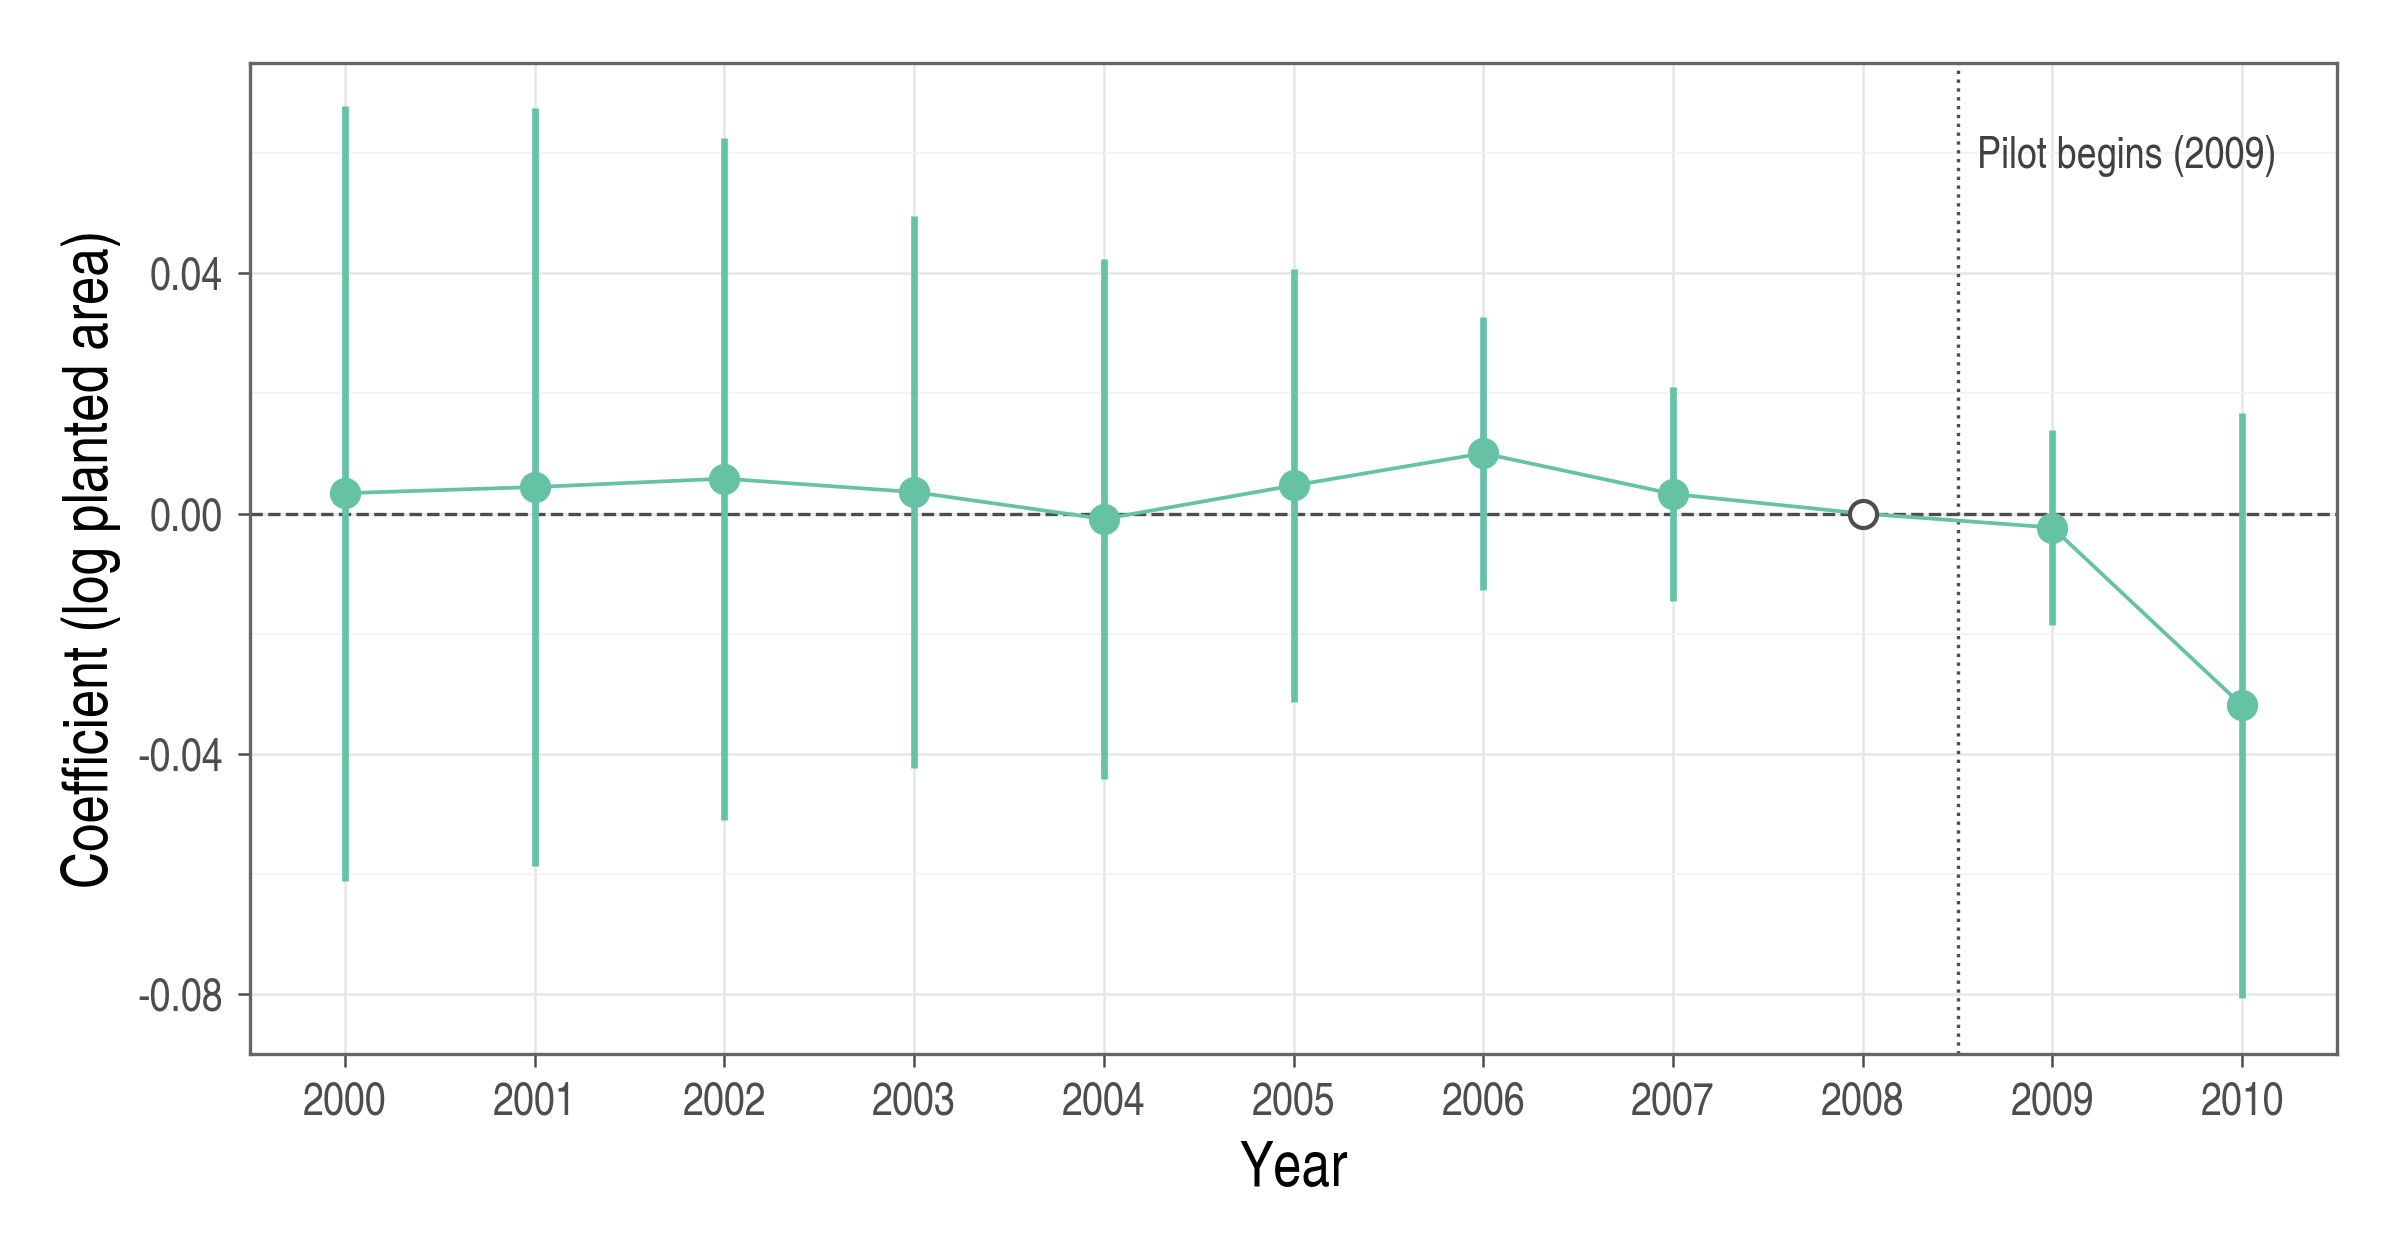
\includegraphics[width=\textwidth]{figures/fig8_rice_event_study.png}
\caption{Event-Study Coefficients for Rice Planted Area, 2000-2010}\label{fig:riceevent}
\notes{Coefficients from a regression of log paddy-rice planted area on municipality and year fixed effects and interactions of early-entry status with year indicators; 2008 is the reference year (open circle). Bars are 95 percent confidence intervals based on municipality-clustered (CR1) standard errors with t(25) critical values; they differ from the wild bootstrap intervals in Table~\ref{tab:rice}. The sample comprises 17 early and nine later-entering municipalities over 2000-2010.}
\end{figure}

\section{Comparability of Treated and Comparison Crops}\label{sec:comparability}

Table~\ref{tab:pregrowth} compares pre-pilot slopes for the seven treated and 22 contributing comparison crops. Mean log-area slopes were \textminus 0.015 and \textminus 0.046 per year, respectively; production slopes were \textminus 0.005 and \textminus 0.031. Yield slopes were closer, at 0.010 and 0.015. Standardized differences are 0.87 for area, 0.71 for production, and \textminus 0.31 for yield. The larger area and production gaps reinforce the pre-pilot divergence in Figure~\ref{fig:eventtime}.

\begin{table}[htbp]
\centering
\caption{Pre-Pilot Growth of Treated and Comparison Crops, 1998-2007}\label{tab:pregrowth}
\begin{tabular*}{\textwidth}{@{\extracolsep{\fill}}lcccc}
\toprule
 & (1) & (2) & (3) & (4) \\
 & \shortstack{Treated\\crops} & \shortstack{Comparison\\crops} & Difference & \shortstack{Std.\\difference} \\
\midrule
Annual growth of cultivated area & \textminus 0.015 & \textminus 0.046 & 0.031    & 0.867 \\
                                 & (0.022)  & (0.045)  &          &  \\
Annual growth of yield           & 0.010    & 0.015    & \textminus 0.005 & \textminus 0.313 \\
                                 & (0.019)  & (0.014)  &          &  \\
Annual growth of production      & \textminus 0.005 & \textminus 0.031 & 0.026    & 0.706 \\
                                 & (0.022)  & (0.046)  &          &  \\
Crop series                      & 7        & 22       &          &  \\
\bottomrule
\end{tabular*}
\notes{Unweighted means of crop-specific least-squares slopes of log outcomes on year over 1998-2007; standard deviations across crops in parentheses. Difference is the treated mean minus the comparison mean. Standardized difference divides that gap by the square root of the average of the two group variances; it is descriptive, not a test statistic. Large and small green onions have eight annual observations; other crops have ten.}
\end{table}

Changing the reference period or comparison pool changes the growth histories against which treated crops are evaluated. The pre-pilot differences help explain the comparisons underlying the national sensitivity results. The municipal design holds crop identity fixed and instead compares regional growth histories.

\chapter{Discussion and Policy Implications}\label{ch:discussion}

\section{Policy Implications}\label{sec:policy}

The three forms of government support address different problems and should be evaluated accordingly. Premium subsidies reduce the price farmers pay for protection, administrative subsidies support its delivery, and state reinsurance shares losses that are difficult to diversify. Production responses provide only one part of this assessment. Access to insurance, the distribution of support, service quality, and public financial exposure are also relevant. Since subsidies and indemnities are transfers, their amounts alone do not measure welfare gains. Those gains depend on risk reduction, changes in behavior, and the cost of raising public funds.

For premium subsidies, the central trade-off is between making coverage affordable and directing public support toward intended beneficiaries. Below the national ceiling, farmers with higher eligible premiums receive larger subsidies. The ceiling limits the size of these transfers but does not distinguish households by their ability to pay. One option is a tapered schedule that reduces the marginal subsidy rate above an insured-value threshold. This would limit support for larger contracts while preserving assistance below the threshold. However, contract size also reflects crop choice, coverage, and risk exposure. The design should therefore consider these factors alongside farm size, household income, and local subsidies. A reduction in expenditure would be more desirable if it reduced large transfers without discouraging coverage among vulnerable farms.

Administrative subsidies raise a different question: whether public payments encourage efficient and reliable service. Cost per active contract and per settled claim would provide useful comparisons across products and regions, particularly when assessed alongside settlement times and corrections to loss assessments. A performance component could reward timely and accurate settlement, while a separate payment could compensate for the cost of serving remote areas. Operating-cost ratios alone are insufficient for this purpose because they also change with premium levels and product complexity.

For state reinsurance, a useful alternative is an arrangement in which private insurers retain ordinary losses and public coverage begins above a catastrophe threshold. Comparing this arrangement with the current mixed system would help clarify the trade-off between private incentives and public capacity to bear risk \citep{mahul2010,jia2025}. Each arrangement should be evaluated under the same loss scenarios, with attention to expected net public cost, severe-year financing needs, private retention, and the price of reinsurance. Catastrophe-focused coverage is not necessarily preferable in every setting. The appropriate threshold depends on how much risk private insurers can retain and the cost of financing that risk.

\section{Climate Risk and the Design of Support}\label{sec:climate}

Climate change matters for insurance through both the scale of losses and the extent to which they occur together. More frequent or severe losses can increase expected claims. Greater regional correlation has a different effect. Holding regional loss distributions fixed, it raises the variance of aggregate losses and can increase exposure to extreme outcomes. Under a purely proportional treaty with a fixed sharing rate, however, it does not change expected ceded claims. Under nonlinear arrangements, changes in dependence can also increase expected reinsurance payments.

These differences matter for public financing. Stress tests should apply the actual treaty to joint regional loss scenarios and distinguish expected net public expenditure from the funds needed during severe or consecutive loss years. Climate risk can also affect premium subsidies: if risk-rated premiums rise, public subsidy expenditure may increase even without a change in subsidy rates, subject to the applicable caps.

\section{Limitations and Future Research}\label{sec:limitations}

The national comparison measures changes following insurance availability using aggregate outcomes for insured and uninsured farms. It cannot separate the production responses of participating farms or show how premium subsidies are distributed across households. Divergent pre-pilot trajectories and uncertainty in small-sample inference further restrict causal interpretation. Crop substitution poses an additional concern. If insurance encourages land to move from comparison crops to insured crops, comparison outcomes may themselves respond to the program. Correlations between crop areas are insufficient to establish whether this occurs.

The municipal rice comparison holds crop identity fixed, but its two-year post-pilot period captures only short-run changes. Local investment and weather may also affect the comparison. In addition, neither analysis isolates the role of expected disaster relief in insurance enrollment or production decisions.

Linked insurance contracts and farm-production records would allow future research to distinguish enrollment, coverage choices, and production responses while addressing selection into insurance. Regional rollout designs would also benefit from clearer evidence on how participating locations and introduction dates were selected. To estimate whether disaster relief discourages insurance enrollment, researchers would need variation in assistance that can be separated from disaster severity. For the fiscal assessment, treaty-level models should incorporate the full loss-sharing rules, joint regional losses, and financing conditions.

\chapter{Conclusion}\label{ch:conclusion}

This thesis assesses three forms of government support for South Korea's crop disaster insurance program: premium subsidies, administrative cost subsidies, and state reinsurance. Each form addresses a different constraint on insurance provision. Their assessment therefore focuses on distinct outcomes: access to insurance and the distribution of subsidies for premium support, cost and service quality for administrative support, and risk allocation and fiscal exposure for reinsurance.

The production comparisons provide limited evidence on how insurance availability changes agricultural production. Across seven annual crops, the mean production contrast is 0.020 log points, with an exploratory 95 percent interval of [\textminus 0.277, 0.317]. Its sign changes with the comparison crops and aggregation weights, while divergent pre-pilot trajectories weaken a causal interpretation. The municipal rice estimate is \textminus 0.021 log points, with a 95 percent interval of [\textminus 0.064, 0.022], and varies with the municipalities included. This comparison holds the crop fixed and shows closer observed pre-pilot trajectories, but covers only two post-introduction years and remains vulnerable to differential local shocks. These estimates establish neither a zero production response nor the absence of moral hazard.

The institutional assessment identifies three priorities: evaluate tapered premium support against distribution and coverage objectives, link administrative payments to comparable measures of cost and service quality, and compare current reinsurance arrangements with a catastrophe-focused alternative. These are options to evaluate, rather than designs shown to be optimal by the production estimates. The broader contribution is to distinguish the purposes of government support and the evidence needed to assess each one. Whether support is well designed depends on who receives protection, how efficiently it is delivered, and how losses are shared between private insurers and the public sector.


% ---------- References ----------
\clearpage
\phantomsection
\addcontentsline{toc}{chapter}{References}
% Reference list (APA style, as in the original document).
% The optional argument of each \bibitem sets the author-year label used
% by \citet / \citep, e.g. \citep{miranda1997} -> (Miranda & Glauber, 1997).
\begingroup
\setstretch{1.3}
\begin{thebibliography}{}

\bibitem[{APFS}(n.d.)]{apfs}
Agricultural Policy Insurance \& Finance Service. (n.d.). \textit{Crop disaster insurance enrollment and payment statistics by year, crop, and province} [Data set]. Public Data Portal. \url{https://www.data.go.kr}

\bibitem[{Callaway \& Sant'Anna}(2021)]{callaway2021}
Callaway, B., \& Sant'Anna, P. H. C. (2021). Difference-in-differences with multiple time periods. \textit{Journal of Econometrics, 225}(2), 200-230. \url{https://doi.org/10.1016/j.jeconom.2020.12.001}

\bibitem[{Cameron et al.}(2008)]{cameron2008}
Cameron, A. C., Gelbach, J. B., \& Miller, D. L. (2008). Bootstrap-based improvements for inference with clustered errors. \textit{Review of Economics and Statistics, 90}(3), 414-427. \url{https://doi.org/10.1162/rest.90.3.414}

\bibitem[{Choi et al.}(2010)]{choi2010}
Choi, K. H., Chae, G. S., \& Yoon, B. S. (2010). \textit{The performance and tasks of crop insurance} (Research Report R615). Korea Rural Economic Institute.

\bibitem[Coate(1995)]{coate1995}
Coate, S. (1995). Altruism, the Samaritan's dilemma, and government transfer policy. \textit{American Economic Review, 85}(1), 46-57.

\bibitem[{Goodwin et al.}(2004)]{goodwin2004}
Goodwin, B. K., Vandeveer, M. L., \& Deal, J. L. (2004). An empirical analysis of acreage effects of participation in the federal crop insurance program. \textit{American Journal of Agricultural Economics, 86}(4), 1058-1077. \url{https://doi.org/10.1111/j.0002-9092.2004.00653.x}

\bibitem[Han(2014)]{han2014}
Han, S. (2014). An empirical analysis on the production and price effect by agricultural disaster insurance. \textit{KDI Journal of Economic Policy, 36}(4), 135-169. \url{https://doi.org/10.23895/kdijep.2014.36.4.135}

\bibitem[{Hazell et al.}(2017)]{hazell2017}
Hazell, P., Sberro-Kessler, R., \& Varangis, P. (2017). \textit{When and how should agricultural insurance be subsidized? Issues and good practices}. World Bank Group. \url{http://documents.worldbank.org/curated/en/330501498850168402}

\bibitem[{Jia et al.}(2025)]{jia2025}
Jia, R., Lin, J., Powers, M. R., \& Wang, H. (2025). Catastrophe risk sharing among individuals, private insurance, and government. \textit{Journal of Risk and Insurance, 92}(2), 263-311. \url{https://doi.org/10.1111/jori.12506}

\bibitem[{Just et al.}(1999)]{just1999}
Just, R. E., Calvin, L., \& Quiggin, J. (1999). Adverse selection in crop insurance: Actuarial and asymmetric information incentives. \textit{American Journal of Agricultural Economics, 81}(4), 834-849. \url{https://doi.org/10.2307/1244328}

\bibitem[{K-water}(n.d.)]{kwater}
K-water. (n.d.). \textit{Nakdong River weir management facilities}. \url{https://www.kwater.or.kr/busi/sub02/facilitiespresent03Page.do?s_mid=1509}

\bibitem[{Kang \& Chung}(2017)]{kang2017}
Kang, S., \& Chung, W. (2017). An evaluation of current government reinsurance program and its improvement strategies for crop insurance. \textit{Korean Journal of Agricultural Economics, 58}(2), 21-48. \url{https://doi.org/10.24997/KJAE.2017.58.2.21}

\bibitem[{Lee \& Jung}(2014)]{leejung2014}
Lee, J., \& Jung, J. H. (2014). Adverse selection and moral hazard in the Korean crop insurance market. \textit{Korean Journal of Agricultural Economics, 55}(1), 29-47.

\bibitem[{Lee \& Kim}(2026)]{leekim2026}
Lee, S., \& Kim, T. (2026). Effects of crop insurance on the output and technical efficiency of fruit farms: A stochastic frontier analysis. \textit{Journal of Rural Development, 49}(1), 1-24. \url{https://repository.krei.re.kr/bitstream/2018.oak/32826/1/RE49-1-01.pdf}

\bibitem[Lusk(2017)]{lusk2017}
Lusk, J. L. (2017). Distributional effects of crop insurance subsidies. \textit{Applied Economic Perspectives and Policy, 39}(1), 1-15. \url{https://doi.org/10.1093/aepp/ppw002}

\bibitem[{MacKinnon et al.}(2023)]{mackinnon2023}
MacKinnon, J. G., Nielsen, M. Ø., \& Webb, M. D. (2023). Cluster-robust inference: A guide to empirical practice. \textit{Journal of Econometrics, 232}(2), 272-299. \url{https://doi.org/10.1016/j.jeconom.2022.04.001}

\bibitem[{MacKinnon \& Webb}(2018)]{mackinnonwebb2018}
MacKinnon, J. G., \& Webb, M. D. (2018). The wild bootstrap for few (treated) clusters. \textit{The Econometrics Journal, 21}(2), 114-135. \url{https://doi.org/10.1111/ectj.12107}

\bibitem[{Mahul \& Stutley}(2010)]{mahul2010}
Mahul, O., \& Stutley, C. J. (2010). \textit{Government support to agricultural insurance: Challenges and options for developing countries}. World Bank. \url{https://doi.org/10.1596/978-0-8213-8217-2}

\bibitem[{Ministry for Food, Agriculture, Forestry and Fisheries}(2011)]{mifaff2011}
Ministry for Food, Agriculture, Forestry and Fisheries. (2011, May 9). \textit{Rice disaster insurance goes on sale from May 11} [Press release].

\bibitem[MAFRA(2024)]{mafra2024}
Ministry of Agriculture, Food and Rural Affairs. (2024). \textit{2024 agricultural insurance yearbook}.

\bibitem[MAFRA(2025)]{mafra2025}
Ministry of Agriculture, Food and Rural Affairs. (2025). \textit{2025 agricultural insurance yearbook}.

\bibitem[MAFRA(2026)]{mafra2026}
Ministry of Agriculture, Food and Rural Affairs. (2026). \textit{2026 crop disaster insurance implementation guidelines}. \url{https://www.mafra.go.kr/bbs/home/798/596394/download.do}

\bibitem[{Miranda \& Glauber}(1997)]{miranda1997}
Miranda, M. J., \& Glauber, J. W. (1997). Systemic risk, reinsurance, and the failure of crop insurance markets. \textit{American Journal of Agricultural Economics, 79}(1), 206-215. \url{https://doi.org/10.2307/1243954}

\bibitem[{Nam \& Ahn}(2022)]{nam2022}
Nam, K., \& Ahn, B. (2022). The effect of purchasing crop insurance on the input utilization and farm income. \textit{Korean Journal of Agricultural Management and Policy, 49}(2), 157-190.

\bibitem[{Nelson \& Loehman}(1987)]{nelson1987}
Nelson, C. H., \& Loehman, E. T. (1987). Further toward a theory of agricultural insurance. \textit{American Journal of Agricultural Economics, 69}(3), 523-531. \url{https://doi.org/10.2307/1241688}

\bibitem[{Raschky \& Weck-Hannemann}(2007)]{raschky2007}
Raschky, P. A., \& Weck-Hannemann, H. (2007). Charity hazard: A real hazard to natural disaster insurance? \textit{Environmental Hazards, 7}(4), 321-329. \url{https://doi.org/10.1016/j.envhaz.2007.09.002}

\bibitem[Roth(2022)]{roth2022}
Roth, J. (2022). Pretest with caution: Event-study estimates after testing for parallel trends. \textit{American Economic Review: Insights, 4}(3), 305-322. \url{https://doi.org/10.1257/aeri.20210236}

\bibitem[{Statistics Korea}(2014)]{statkorea2014}
Statistics Korea. (2014). \textit{Regular statistical quality assessment of the Crop Production Survey: Final report}.

\bibitem[{Statistics Korea}(n.d.)]{statkorea_nd}
Statistics Korea. (n.d.). \textit{Crop Production Survey} [Data set]. Korean Statistical Information Service. \url{https://kosis.kr}

\bibitem[Webb(2023)]{webb2023}
Webb, M. D. (2023). Reworking wild bootstrap-based inference for clustered errors. \textit{Canadian Journal of Economics, 56}(3), 839-858. \url{https://doi.org/10.1111/caje.12661}

\bibitem[{Yu et al.}(2018)]{yu2018}
Yu, J., Smith, A., \& Sumner, D. A. (2018). Effects of crop insurance premium subsidies on crop acreage. \textit{American Journal of Agricultural Economics, 100}(1), 91-114. \url{https://doi.org/10.1093/ajae/aax058}

\end{thebibliography}
\endgroup


% ---------- Appendix ----------
\appendix
\chapter{National Inference and Crop Influence}\label{app:inference}

% Appendix numbering: equations (A1), (A2); Table A1
\setcounter{equation}{0}
\setcounter{table}{0}
\setcounter{figure}{0}
\renewcommand{\theequation}{A\arabic{equation}}
\renewcommand{\thetable}{A\arabic{table}}
\renewcommand{\thefigure}{A\arabic{figure}}

The contrast is linear in the log outcomes and can be written as $\widehat{\theta} = \sum_{c,t}a_{ct}\, y_{ct}$. Crop and year fixed effects fitted on unexposed observations provide residuals $\widehat{u}_{ct}$, and treated post-period residuals are centered by their event-year contrast. The crop-level score and analytic standard error are
\begin{equation}\label{eq:score}
\psi_{c} = \sum_{t}a_{ct}\,\widehat{u}_{ct},\qquad SE_{score} = \sqrt{\frac{G}{G - 1}\sum_{c}\psi_{c}^{2}},
\end{equation}
where $G$ is the number of contributing crop series. In each of 9,999 draws, one multiplier per crop is drawn with equal probability from Webb's \citeyearpar{webb2023} six-point distribution,
\begin{equation}\label{eq:webb}
v_{c} \in \left\{ -\sqrt{3/2},\, -1,\, -\sqrt{1/2},\,\sqrt{1/2},\, 1,\,\sqrt{3/2} \right\}.
\end{equation}

The multiplier statistic sums crop scores multiplied by their draws. The interval adds and subtracts the 95th percentile of its absolute value from the estimated contrast. The p-value is the share of draws whose absolute value is at least as large as the estimate, with a plus-one adjustment. Area-weighted and event-time statistics replace cell weights with those implied by equation~\eqref{eq:areaweights} and the event-time comparisons, using the same residuals and draws. The joint pre-pilot test compares the sum of squared standardized contrasts with its distribution across these draws. Independent multipliers preserve within-crop dependence but not residual dependence across crops. This score procedure differs from the null-imposed, studentized regression bootstrap used for rice; the use of Webb weights does not establish its finite-sample validity.

\begin{table}[htbp]
\centering
\caption{Leave-One-Crop-Out Contrasts}\label{tab:leaveoneout}
\begin{tabular*}{0.8\textwidth}{@{\extracolsep{\fill}}lccc}
\toprule
Omitted crop & (1) & (2) & (3) \\
             & Area & Yield & Production \\
\midrule
Soybean       & 0.078    & \textminus 0.061 & 0.017 \\
Onion         & \textminus 0.007 & \textminus 0.037 & \textminus 0.044 \\
Sweet potato  & 0.020    & \textminus 0.019 & 0.000 \\
Corn          & 0.066    & \textminus 0.044 & 0.022 \\
Garlic        & 0.050    & \textminus 0.028 & 0.022 \\
Spring potato & 0.003    & \textminus 0.012 & \textminus 0.009 \\
Red pepper    & 0.129    & 0.003    & 0.132 \\
\bottomrule
\end{tabular*}
\notes{Log-point contrasts with six treated crops, the full comparison pool, the last pre-pilot reference year, and event years 0-9. Omitted crops are not added to the comparison pool.}
\end{table}


\end{document}
